\documentclass[10pt,a4paper]{article}
\usepackage[latin1]{inputenc}
% \usepackage{amsmath}
\usepackage{amsfonts}
% \usepackage{amssymb}
\usepackage{amsmath,amsthm,amssymb}
\usepackage{graphicx}
\usepackage{hyperref}
% \usepackage{courier}
\usepackage{placeins}
\usepackage{fancyhdr}
\usepackage{color}
% \usepackage{xcolor}
\usepackage{listings}
\usepackage{geometry}
\usepackage{tabularx}
\usepackage[table]{colortbl}
\usepackage{placeins}
% \usepackage{cite}
\usepackage{subcaption}
\usepackage{lipsum}
\usepackage{titlesec}
\usepackage{dsfont}
\usepackage{parskip}
\usepackage{soul}
\usepackage[backend=biber]{biblatex}
\addbibresource{mybib.bib}
\usepackage[skip=8pt,labelfont=bf, font=sf]{caption}
	\DeclareCaptionFont{myfont}{\fontfamily{\sfdefault}\selectfont}

\hypersetup{
	colorlinks   = True,
	citecolor    = blue,
	linkcolor	 = blue,
}

% \geometry{letterpaper, portrait, margin=1in}
% \geometry{a4paper,margin=15mm,bindingoffset=25mm,heightrounded,}
\geometry{a4paper,margin=25mm}

\usepackage[dvipsnames]{xcolor}
\definecolor{lightgray}{rgb}{.93,.93,.93}
\definecolor{darkgray}{rgb}{.4,.4,.4}
\definecolor{purple}{rgb}{0.65, 0.12, 0.82}

\usepackage{helvet}
\usepackage{times}

\titleformat{\chapter}[display]
  {\normalfont\sffamily\huge\bfseries} % \color{blue}
  {\chaptertitlename\ \thechapter}{20pt}{\Huge}
\titleformat{\section}
  {\normalfont\sffamily\huge\bfseries} % \color{cyan}
  {\thesection}{1em}{}
 \titleformat{\subsection}
  {\normalfont\sffamily\Large\bfseries} % \color{cyan}
  {\thesubsection}{1em}{}
 \titleformat{\subsubsection}
  {\normalfont\sffamily\large\bfseries} % \color{cyan}
  {\thesubsubsection}{1em}{}
\renewenvironment{abstract}
 {\par\noindent\Huge\textbf{\abstractname.}\\\vspace{1em}\ignorespaces}
 {\par\medskip} 

% \renewcommand*\abstractname{Abstract\hfill}
% \renewcommand{\familydefault}{\sfdefault}


\def \lineheight {1.5pt}

\makeatletter
   \def\vhrulefill#1{\leavevmode\leaders\hrule\@height#1\hfill \kern\z@}
\makeatother

\usepackage{caption}
    \DeclareCaptionType{mycapequ}[][List of equations]
    \captionsetup[mycapequ]{labelformat=empty}

\usepackage{inconsolata}

\lstset{
	language=Matlab,
	backgroundcolor=\color{lightgray},
	keywordstyle=\color{blue}\bfseries,
	stringstyle=\color{red}\ttfamily,
	commentstyle=\color{ForestGreen}\ttfamily,
	identifierstyle=\color{black},
	extendedchars=true,
	% basicstyle=\footnotesize\ttfamily,
	basicstyle=\normalsize\fontencoding{T1}\ttfamily,
	showstringspaces=false,
	showspaces=false,
	numbers=left,
	numberstyle=\footnotesize,
	numbersep=9pt,
	tabsize=2,
	breaklines=true,
	showtabs=false,
	captionpos=b
}

\lstset{
	language=Python,
	backgroundcolor=\color{lightgray},
	keywordstyle=\color{blue}\bfseries,
	stringstyle=\color{red}\ttfamily,
	commentstyle=\color{ForestGreen}\ttfamily,
	identifierstyle=\color{black},
	extendedchars=true,
	% basicstyle=\footnotesize\ttfamily,
	basicstyle=\normalsize\fontencoding{T1}\ttfamily,
	showstringspaces=false,
	showspaces=false,
	numbers=left,
	numberstyle=\footnotesize,
	numbersep=9pt,
	tabsize=2,
	breaklines=true,
	showtabs=false,
	captionpos=b
}

\fancypagestyle{firstpage}{%
  \fancyhf{}% clear default for head and foot
  % \rfoot{\textbf{Page \thepage}}
  % \lfoot{\textbf{\today}}
  \renewcommand{\headrulewidth}{0pt}
}
\fancypagestyle{blank}{%
	\fancyhf{}
	\renewcommand{\headrulewidth}{0pt}
}

\fancypagestyle{nohdr}{%
	\fancyhf{}
	\renewcommand{\headrulewidth}{0pt}
	\rfoot{\fontfamily{\sfdefault}\selectfont\textbf{Page \thepage}}
}

\renewcommand{\headrulewidth}{1pt}% 2pt header rule


% \fontfamily{\sfdefault}\selectfont
	% \large\fontfamily{\rmdefault}\selectfont 

\setlength{\parskip}{12pt} % 1ex plus 0.5ex minus 0.2ex}
\setlength{\parindent}{0pt}

\DeclareMathOperator*{\argmin}{argmin}

\pagestyle{fancy}
% \renewcommand{\sectionmark}[1]{\markboth{ #1}{}}
% \renewcommand{\subsectionmark}[1]{\markboth{\thesection\ #1}{\thesubsection\ #1}}
\fancyhf{}
\rhead{\fontfamily{\sfdefault}\selectfont \textbf{\rightmark}}
\lhead{\fontfamily{\sfdefault}\selectfont \textbf{Specialization Project}}
\rfoot{\fontfamily{\sfdefault}\selectfont \textbf{Page \thepage}}
\lfoot{\fontfamily{\sfdefault}\selectfont \textbf{Cole Nielsen}} % \today

\title{\textbf{}}
\date{}

\sloppy\raggedright
\begin{document}	
		% \maketitle 
	% \renewcommand{\familydefault}{\sfdefault}
	\thispagestyle{firstpage}
	\fontfamily{\sfdefault}\selectfont 
	\includegraphics[width=0.5\linewidth]{logo_ntnu_eng_black.png} \\
	\vspace{8em}
	\huge Python Framework for Design and Simulation of Integer-N ADPLLs\\	
	\vspace{3em}
	\huge \textbf{Cole Nielsen}\\
	\vspace{14em}
	\large
	Electronic Systems Design, Specialization Project\\
	\vspace{4pt}
	\FloatBarrier

	\def\arraystretch{1.3}
	\setlength{\tabcolsep}{1em}
	\begin{tabular}{@{} l  l}
	Submission date: & December 2019\\
	Supervisor: & Trond Ytterdal, IET\\
	Co-supervisor: & Carsten Wulff, IET\\
	\end{tabular} \\
	\FloatBarrier
	\vspace{3em}
	Norwegian University of Science and Technology \\ 
	\vspace{4pt}Department of Electronic Systems\\
	
	% \begin{center}
	% 	\large
	% 	\begin{tabular}{ l r }
	% 		\textbf{Name} & Cole Nielsen \\
	% 		\textbf{Assigned N$^\textbf{\textnormal{o}}$} & 13 \\
	% 		\textbf{Term} & Autumn 2018\\
	% 		\textbf{Instructor} & Guennadi Kouzaev\\
	% 	\end{tabular}
	% \end{center}
	% \vspace{2em}
	% \vhrulefill{\lineheight}
	\pagebreak
	\thispagestyle{blank}
	\null\pagebreak

	% % % % % % % % % % % % % % % % % % % % % % % % % % % % % % % % % % % % 
	% Abstract		
	\setcounter{page}{1}
	\pagebreak
	\thispagestyle{nohdr}
	\begin{abstract}
		\large\fontfamily{\rmdefault}\selectfont 
		An open source Python-language design automation and simulation framework for the design of integer-N all digital phase locked loop (ADPLL) frequency synthesizers is presented in this paper. The framework enables (1) automatic design of optimized second order discrete time digital loop filters, and (2) behavioral ADPLL simulation to verify loop filter and PLL designs for satisfactory phase noise, lock-time and stability; optionally subject to variation using Monte-Carlo sampling. Simulation is implemented with a discrete-event time domain simulator utilizing behavioral PLL component models, permitting accurate modeling of effects of time-discretization and quantization in an ADPLL. Loop filter design automation is based upon a prototype second order filter, whose parameters are optimized to minimize total integrated output phase noise for a PLL provided specifications for reference frequency, divider ratio, time-to-digital converter (TDC) resolution, digitally controlled oscillator (DCO) gain, oscillator phase noise characteristics and maximum lock time. The optimizer utilizes continuous phase transfer function approximation of ADPLL dynamics and phase noise, which allows for computationally fast evaluation, but also requires conversion of the design filters from continuous-to-discrete time. Second order optimization is utilized post filter design to map the discrete filter into a fixed-point digital with acceptable quantization noise and filter error due to quantization effects.
	\end{abstract}
	% \section*{Abstract}
	% fjdsfkajjlkf

	% % % % % % % % % % % % % % % % % % % % % % % % % % % % % % % % % % % % 
	% Project Description
	\pagebreak
	\thispagestyle{nohdr}
	\null\pagebreak
	\thispagestyle{nohdr}
	\Huge\textbf{Problem description.}\\
	\vspace{1em}
	\large\fontfamily{\rmdefault}\selectfont 
	
	The intent of this project is to develop a standalone PLL design and simulation framework to aid and facilitate a later master's thesis project regarding the design of an all-digital, ultra-low power PLL frequency synthesizer. This framework is intended to address and ease all-digital PLL design and simulation challenges at a high level. Specifically it should enable speedy PLL simulation defined with system and component- level specifications (e.g. desired frequency, gain of digitally controlled oscillator, phase detector resolution, divider ratio). This is to allow for development of component level specifications and verification of PLL performance (phase noise, lock time, stability) under ideal circumstances before transistor level implementation, thus accelerating overall implementation time for hardware.

	% % % % % % % % % % % % % % % % % % % % % % % % % % % % % % % % % % % % 
	% % Preface
	% \pagebreak
	% \thispagestyle{nohdr}
	% \null\pagebreak
	% \thispagestyle{nohdr}
	% \large\fontfamily{\sfdefault}\selectfont 
	% \Huge\textbf{Preface.}\\
	% \vspace{1em}
	% \large\fontfamily{\rmdefault}\selectfont 
	% \lipsum[1]

	% % % % % % % % % % % % % % % % % % % % % % % % % % % % % % % % % % % % 
	% Contents, list of tables and figures
	\fontfamily{\sfdefault}\selectfont 
	\thispagestyle{nohdr}
	\null\pagebreak
	\thispagestyle{nohdr}
	\null\pagebreak
	\tableofcontents
	\pagebreak
	\listoffigures
	\listoftables

	% \vhrulefill{\lineheight}

	\fontfamily{\rmdefault}\selectfont 
	% % % % % % % % % % % % % % % % % % % % % % % % % % % % % % % % % % % % 
	% Abbreviations
	\pagebreak
\null
\pagebreak
\section*{Abbreviations.}
	\begin{tabular}{@{}ll}
		\textbf{\textsf{ADPLL}}	&	All digital phase locked loop \\
		\textbf{\textsf{BER}}	&	Bit error rate \\
		\textbf{\textsf{BFGS}}	&	Broyden-Fletcher-Goldfarb-Shanno \\
		\textbf{\textsf{BW}}	&	Bandwidth \\
		\textbf{\textsf{CMOS}}	&	Complementary metal oxide semiconductor \\
		\textbf{\textsf{DCO}}	&	Digitally controlled oscillator \\
		\textbf{\textsf{DIV}}	&	Divider \\
		\textbf{\textsf{DNL}}	&	Differential non-linearity \\
		\textbf{\textsf{FFT}}	&	Fast Fourier transform \\
		\textbf{\textsf{FM}}	&	Frequency modulation \\
		\textbf{\textsf{IIR}}	&	Infinite impulse response \\
		\textbf{\textsf{ISM}}	&	Industrial, scientific and medicine \\
		\textbf{\textsf{LF}}	&	Loop filter \\
		\textbf{\textsf{LSB}}	&	Least signigicant bit \\
		\textbf{\textsf{OTW}}	&	Oscillator tuning word \\
		\textbf{\textsf{PD}}	&	Phase detector \\
		\textbf{\textsf{PI}}	&	Propotional-integral \\
		\textbf{\textsf{PID}}	&	Proportional-integral-derivative \\
		\textbf{\textsf{PLL}}	&	Phase locked loop \\
		\textbf{\textsf{PN}}	&	Phase noise \\
		\textbf{\textsf{PSD}}	&	Power spectral density \\
		\textbf{\textsf{PVT}}	&	Process, voltage and temperature \\
		\textbf{\textsf{RMS}}	&	Root mean squared \\
		\textbf{\textsf{SSB}}	&	Single side band \\
		\textbf{\textsf{TDC}}	&	Time to digital converter \\
		\textbf{\textsf{TF}}	&	Transfer function \\
		\textbf{\textsf{VCO}}	&	Voltage controlled oscillator \\
	\end{tabular}


	% % % % % % % % % % % % % % % % % % % % % % % % % % % % % % % % % % % % 
	\pagebreak
	\FloatBarrier

	\section{Introduction}\label{intro}
	Phase locked loops are extraordinarily useful frequency synthesizers that are vital to the operation of virtually all wired and wireless communication systems of today. The trend towards increasingly lower power wireless devices poses an acute need to reduce PLL power consumption. This is a challenge as PLLs typically rank among the highest power consuming components of a radio, and are necessarily so to limit oscillator phase noise. A sampling of literature on ultra-low power 2.4GHz radios finds oscillator power consumption as a portion of total radio consumption to be 53\% for the receiver in \cite{regulagadda_2018}, 88\% of the transmitter in \cite{shi_2019}, 52\% of the transmitter in \cite{chen_2019}, and 50\% of the receiver in \cite{pengg_2013}. Reducing analog PLL power consumption can be a prohibitive challenge as the performance of analog loop filters degrade as a result of unavoidably lower charge pump current. However, recent CMOS process nodes with minimum gate lengths as small as 7nm allow for all-digital loop filters and PLLs to be a possible alternative to analog designs due to increasingly low power consumption associated with their implementation. Digital loop-filters have the unique advantage where they can be scaled indefinitely as process nodes advance, suffering no loss in performance, while also having greatly reduced sensitivities to process, voltage, temperature (PVT) variations compared to analog implementations.

All-digital PLLs (ADPLLs) introduce new challenges in the process of design in the ultra-low power domain. Low power design is complemented by low complexity design, which in a PLL transcribes to low resolution of phase detectors, digitally tunable oscillators, and loop filter digital data paths. In other words, effects of quantization are strong. Quantization is an inherently nonlinear process, thus strong quantization is tied to strong nonlinear effects. Consequently, where high resolution digital PLLs with low quantization effects can be effectively analyzed with linear-time invariant transfer functions in the Z-domain, simulation and numerical analysis is necessary to accurately capture quantization effects in low power, low resolution ADPLLs. This, of course, presents a challenge in manual loop filter design of PLLs if simulation is an integral part of the most basic modeling, and thus motivates the creation of an automated design solution. Currently, no openly available PLL design framework automates loop filter design for the needs of ultra low power all-digital PLLs as characterized here. 
% Of the most prominent pre-existing frameworks, CppSim \hl{[add reference...]} features a utility for design of continuous loop filters, however for this it does not provide any level of performance optimization, nor does it support discrete-time and quantized digital designs. 

Thus, in this paper, a new framework, \texttt{pllsim}, written in Python\footnote{Python Software Foundation \url{https://www.python.org/}.} is introduced (this framework is available on GitHub\footnote{\texttt{pllsim} codebase: \url{https://github.com/nielscol/pllsim}.}), which uniquely addresses issues of ultra-low power ADPLL design. Specifically, design of integer-N type PLLs is focused on, as the impetus of this work is an integer-N PLL design project. Topics presented are (a) automatic design and optimization of ADPLL loop filters given target system and component level specifications for the PLL, and (b) behavioral time domain PLL simulation for accurate analysis and verification of loop filter and PLL performance, with an integrated Monte-Carlo sampling variation analysis engine. Due to high phase noise associated with low power design, the optimization approach introduced in this paper focuses on the minimization of total integrated phase noise power to allow for maximum PLL performance on a given power budget.

A brief outline of the paper is as follows. An introduction to PLL theory is in section \ref{theory}. Simulation and optimization methods are discussed in sections \ref{pll_arch}, \ref{methods_lf_design_approach}, \ref{simulator} and \ref{methods_lf_opt}. An example design exercise with the framework, a comparison to existing solutions, and general discussion considerations for using the framework are in section \ref{disco}. Finally, section \ref{conclusion} concludes.
\vspace{1em}

The main contributions of this design framework to PLL design are:
\vspace{-0.8em}
\begin{enumerate}[itemsep=0pt,label=\protect\mycirc{\arabic*}]
	\setlength\itemsep{-0.8em}
	\item Fully automatic loop filter design and optimization for all digital integer-N PLLs in an open source Python framework.
	\item Generation of ready-for-hardware digital filter coefficients from high level PLL specifications (maximum lock time, reference frequency, DCO gain, divider ratio, oscillator phase noise). 
	\item Filter design optimization considering minimization of total phase noise, lock time and quantization errors in the final digital loop filter computed.
	\item An integrated behavioral time domain simulator coupled with the loop filter designer allowing for verification of automatically designed filters for lock time and phase noise performance.
	\item Included parametric sweep and variational analysis in the simulator to verify process tolerance ranges and statistical distributions of PLL performance with process variation.
\end{enumerate}

	\pagebreak
	\FloatBarrier

	\section{Theory}\label{theory}
	
	In its most basic form, a phase locked loop is a phase-based feedback system whose output tracks or maintains a fixed phase relationship to an input signal. As will be shown, such a system is uniquely suited to the task of frequency synthesis, which is the process of generating derivative frequencies from some reference frequency. Given reference and output phase signals $\Phi_{ref}$ and $\Phi_{out}$, a PLL can be modeled as in figure \ref{fig:basic_fb}, with feedforward and feedback networks A(s) and B(s). 
	\begin{figure}[htb!]
		\center\fontfamily{\sfdefault}\selectfont
% XCircuit output "basic_feedback.tex" for LaTeX input from basic_feedback.ps
\def\putbox#1#2#3#4{\makebox[0.00000in][l]{\makebox[#1][l]{}\raisebox{\baselineskip}[0.00000in][0.00000in]{\raisebox{#2}[0.00000in][0.00000in]{\scalebox{#3}{#4}}}}}
\def\rightbox#1{\makebox[0.00000in][r]{#1}}
\def\centbox#1{\makebox[0.00000in]{#1}}
\def\topbox#1{\raisebox{-0.60\baselineskip}[0.00000in][0.00000in]{#1}}
\def\midbox#1{\raisebox{-0.20\baselineskip}[0.00000in][0.00000in]{#1}}
   \scalebox{1}{
   \normalsize
   \parbox{3.61667in}{
   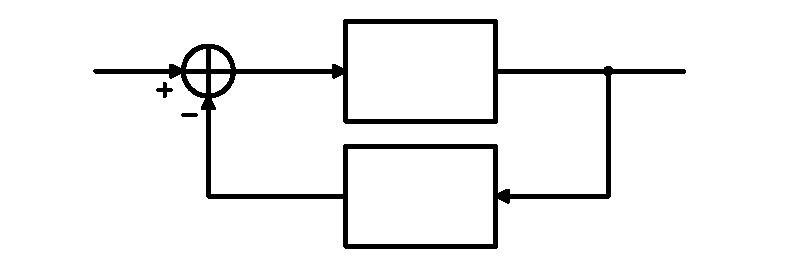
\includegraphics[scale=0.70000]{./figs/basic_feedback.pdf}\\
   % translate x=544 y=496 scale 0.38
   \putbox{1.82000in}{0.85400in}{1.20}{A(s)}%
   \putbox{1.82000in}{0.27300in}{1.20}{B(s)}%
   \putbox{0.44800in}{1.00100in}{1.20}{$\Phi_{ref}$}%
   \putbox{2.84200in}{1.00100in}{1.20}{$\Phi_{out}$}%
   \putbox{1.12000in}{1.00100in}{1.20}{$\Phi_{error}$}%
   } % close 'parbox'
   } % close 'scalebox'
   \vspace{-\baselineskip} % this is not necessary, but looks better
\fontfamily{\rmdefault}\selectfont

		\caption{Basic phase feedback network.}
		\label{fig:basic_fb}
	\end{figure}
	\FloatBarrier
	The closed loop phase response T(s) for $\Phi_{ref}$ to $\Phi_{out}$ is therefore:
	\begin{equation}
		\mathrm{T}(s) = \frac{\Phi_{out}(s)}{\Phi_{ref}(s)} = \frac{A(s)}{1+A(s)B(s)}
	\end{equation}
	A particular case of interest is when B(s) = 1/N, where N is a constant, and the loop gain A(s)B(s) $>>$ 1, the closed loop response is:
	\begin{equation}\label{mult_by_n}
		\frac{\Phi_{out}(s)}{\Phi_{ref}(s)} \approx \frac{A(s)}{A(s)B(s)} = \frac{1}{B(s)} = N
	\end{equation}
	We see that the phase through the PLL is multiplied by a factor of N. If the input phase signal is a sinusoid with frequency $\omega_{ref}$, and likewise the output with $\omega_{out}$, then $\phi_{ref}(t)=\omega_{ref}t$ and $\phi_{out}(t)=\omega_{out}t$. Thus:
	\begin{equation}\label{mult_by_n}
		\frac{\Phi_{out}(t)}{\Phi_{ref}(t)} = \frac{\omega_{out}t}{\omega_{ref}t} \approx N \hspace{1em} \rightarrow \hspace{1em} \omega_{out} \approx N\omega_{ref}
	\end{equation}
	Therefore, it is observed that a PLL allows for the generation, i.e. synthesis, of a new frequency from a reference frequency signal. Given a feedback divider ration of 1/N, the PLL multiplies the reference frequency by a factor of N. In the following sections, more advanced models for PLL will be developed, extending the concept introduced here. Specifically, the theory of digital, discrete-time PLLs will be developed and extended from a continuous phase model of a basic PLL.

	\subsection{Continuous PLL Model}
		Although PLLs are practically limited to using discrete-time sampling in real-word hardware, continuous models can still be applied in their analysis and design. Thus a continuous PLL model is developed in this section to aid in the later discussed discretized PLL modeling.

		\subsubsection{PLL Synthesizer architecture}
			The traditional architecture for implementing a PLL frequency synthesizer \cite{Razavi1996DesignOM} is shown in figure \ref{fig:basic_pll}. This basic PLL is comprised of four components: (1) a phase detector, denoted by PD, (2) a loop filter, denoted by H$_{LF}$(s), (3) a voltage controlled oscillator, denoted by VCO, and (4) and phase divider, denoted by "$\div$ N" in the figure. These components are explained in the following sections.
			\begin{figure}[htb!]
				\center\fontfamily{\sfdefault}\selectfont
% XCircuit output "basic_pll.tex" for LaTeX input from basic_pll.ps
\def\putbox#1#2#3#4{\makebox[0.00000in][l]{\makebox[#1][l]{}\raisebox{\baselineskip}[0.00000in][0.00000in]{\raisebox{#2}[0.00000in][0.00000in]{\scalebox{#3}{#4}}}}}
\def\rightbox#1{\makebox[0.00000in][r]{#1}}
\def\centbox#1{\makebox[0.00000in]{#1}}
\def\topbox#1{\raisebox{-0.60\baselineskip}[0.00000in][0.00000in]{#1}}
\def\midbox#1{\raisebox{-0.20\baselineskip}[0.00000in][0.00000in]{#1}}
   \scalebox{1}{
   \normalsize
   \parbox{4.49167in}{
   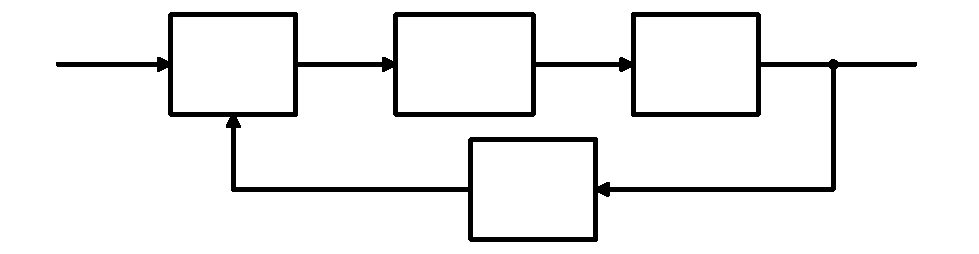
\includegraphics[scale=0.70000]{./figs/basic_pll.pdf}\\
   % translate x=320 y=488 scale 0.38
   \putbox{0.97300in}{0.82600in}{1.20}{PD}%
   \putbox{2.34500in}{0.24500in}{1.20}{$\div$ N}%
   \putbox{0.32900in}{0.97300in}{1.20}{$\Phi_{ref}$}%
   \putbox{3.71700in}{0.97300in}{1.20}{$\Phi_{out}$}%
   \putbox{1.90400in}{0.82600in}{1.20}{H$_{LF}$(s)}%
   \putbox{3.07300in}{0.82600in}{1.20}{VCO}%
   \putbox{1.49800in}{0.39200in}{1.20}{$\Phi_{div}$}%
   \putbox{1.52600in}{0.97300in}{1.20}{$\Phi_e$}%
   \putbox{2.54800in}{0.97300in}{1.20}{V$_{ctrl}$}%
   } % close 'parbox'
   } % close 'scalebox'
   \vspace{-\baselineskip} % this is not necessary, but looks better
\fontfamily{\rmdefault}\selectfont

				\caption{Basic PLL.}
				\label{fig:basic_pll}
			\end{figure}
			\FloatBarrier

		\subsubsection{Divider}
			The phase divider is used as the feedback path in the PLL, where the division modulus N controls the frequency multiplication of the PLL. The tranfer function of the divider is:
			\begin{equation}
				\mathrm{H}_{div}(s) = \frac{\Phi_{div}(s)}{\Phi_{out}(s)} = \frac{1}{\mathrm{N}}
			\end{equation}

			\subsubsection{Phase detector}
			The phase detector is used to measure the phase of the feedback signal (i.e. divider output) in relation to the reference phase, in order to establish a phase error signal $\Phi_e$ used to control the tuning of the PLL.
			\begin{equation}
				\Phi_e(s) = \Phi_{ref}(s) - \Phi_{div}(s)
			\end{equation}

		\subsubsection{Loop Filter}
			The PLL loop filter is used to control the phase-frequency response of PLL, which affects transient PLL behavior, as well as phase noise performance (see section \ref{pn_theory}). As will later be seen, low pass response is desired in a PLL, so the loop filter must be designed accordingly. Generally, this can be designed arbitrarily to have P poles and Z zeros, as such:
			\begin{equation}
				\textnormal{H}_{LF}(s) = \frac{\Sigma_0^Z b_js^j}{\Sigma_0^P a_ks^k}
			\end{equation}
			Rational choice of the loop filter will ensure that the PLL will be stable and minimize steady state phase error. In order to achieve zero steady state error, the loop filter must contain a pole at zero, in other words an integrator. A PLL containing such a pole is classified as a Type II PLL, and a PLL omitting the pole is considered Type I. A logical approach to loop filter design for zero-phase error is to treat it as a PID controller, where:
			\begin{equation}
				\textnormal{H}_{LF}(s) = sK_d + K_p + \frac{K_i}{s} = \frac{K_d}{s}\left(s^2 + s\frac{K_p}{K_d} + \frac{K_i}{K_d}\right)
			\end{equation}
			Such a loop filter contains two zeros and one integrator pole at zero. The gain parameters $K_p, K_i, K_d$ can be tuned to achieve the desired bandwidth and stability for the PLL. The impacts of loop filter design will be further considered in sections \ref{cont_pll_tf}-\ref{other_pid}.
			
		\subsubsection{VCO}
			The voltage controlled oscillator is an oscillator with frequency controlled by an input signal V$_{ctrl}$. The VCO is characterized by its gain $K_{DCO} = \partial f/\partial \textnormal{V}_{ctrl}$, and the nominal oscillation frequency $f_0$. Analyzed in terms of phase, an oscillator can be seen as a time-phase integrator:
			\begin{equation}
				\Phi_{VCO}(t) = \Phi_{out}(t) = \int2\pi(K_{DCO}\textnormal{V}_{ctrl}(t) + f_0)\mathrm{dt}
			\end{equation}
			In s-domain, where frequency offsets will be represented via initial conditions for modeling purposes, the VCO transfer function is therefore:
			\begin{equation}
				\mathrm{H}_{VCO}(s) = \frac{\Phi_{VCO}(s)}{\textnormal{V}_{ctrl}(s)} = \frac{\Phi_{out}(s)}{\textnormal{V}_{ctrl}(s)} = \frac{2\pi K_{DCO}}{s}
			\end{equation}

		\subsubsection{Continuous PLL Transfer function}\label{cont_pll_tf}
			Now that the continuous PLL synthesizer is understood at a component level, the closed loop dynamics of the PLL can be analyzed. First the PLL loop gain is determined:
			\begin{equation}
				\mathrm{L}(s) = \textnormal{H}_{LF}(s)\textnormal{H}_{VCO}(s)\textnormal{H}_{div}(s) = \frac{2\pi K_{VCO}K_d}{\mathrm{N}}\frac{1}{s^2}\left(s^2 + s\frac{K_p}{K_d} + \frac{K_i}{K_d}\right)
			\end{equation}
			With the phase detector as the feedback summation point, the closed loop response of the PLL from reference to output is:
			\begin{align} \label{eq:pid_pll_tf}
				\mathrm{T}(s) = \frac{\Phi_{out}(s)}{\Phi_{ref}(s)} = \frac{2\pi K_{VCO}\left(s^2K_d + sK_p + K_i\right)}{s^2\left(1 + \frac{2\pi K_{VCO}K_d}{\mathrm{N}}\right) + \frac{2\pi K_{VCO}}{\mathrm{N}}\left(sK_p + K_i\right)} = \mathrm{N}\frac{\mathrm{L}(s)}{1 + \mathrm{L}(s)}
			\end{align}
			It should be noted that in the closed loop configuration, this PLL phase transfer function contains two poles and two zeros. This is not a low pass response as desired for a satisfactory PLL phase noise power spectrum, as will later be discussed. In order achieve low pass operation, the derivative term $K_d$ must be set to zero, yielding a PI controller for the loop filter (with one zero and two poles):
			\begin{align} \label{eq:full_pi_pll_tf}
				\mathrm{T}(s) = \frac{\Phi_{out}(s)}{\Phi_{ref}(s)} = \frac{2\pi K_{VCO}\left(sK_p + K_i\right)}{s^2 + \frac{2\pi K_{VCO}}{\mathrm{N}}\left(sK_p + K_i\right)} = \mathrm{N}\frac{\mathrm{L}(s)}{1 + \mathrm{L}(s)} 
			\end{align}
			Steady state zero phase error can be verified by solving the closed loop $\Phi_e(s)$ for s=0:
			\begin{align}
				\left.\Phi_e(s)\right\vert_{s=0} = \left(\Phi_{ref}(0) - \frac{\Phi_{out}(0)}{\mathrm{N}}\right) = \Phi_{ref}(0)\left(1 - \frac{\Phi_{out}(0)}{\mathrm{N}\Phi_{ref}(0)}\right)= \Phi_{ref}(0)\left(1 - \frac{\mathrm{N}}{\mathrm{N}}\right) = 0
			\end{align}

		\subsubsection{PI-loop filter design}
			Given a PI-controller loop filter, which can be optionally represented using a pole at zero and a zero with $\omega_z = K_i/K_p$:
			\begin{equation} \label{eq:pi_pll_tf}
				\textnormal{H}_{LF}(s) = K_p + \frac{K_i}{s}  = \frac{K_i}{s}\left(\frac{s}{\omega_z} + 1\right) 
			\end{equation}
			Selection of (not-necessarily optimal) PI controller gains can be easily derived from overall PLL settling time requirements. Suppose that settling time $t_s$ is defined such that the PLL settles within $\pm \delta$ of the final value for a step input. If the initial and final PLL output frequencies are $f_i$ and $Nf_{ref}$, and settling with $\pm f_{tol}$ is desired,  $\delta = f_{tol}/|f_i - Nf_{ref}|$. Setting time is therefore:
			\begin{equation}
				t_s = -\tau\ln(\delta)
			\end{equation}
			Thus, to find settling time, a value for the PLL time constant $\tau$ must be derived. Rewriting equation \ref{eq:full_pi_pll_tf} with substitutions $\omega_z = K_i/K_p$ and $\mathrm{K} = 2\pi K_{VCO}K_i/\mathrm{N}$:
			\begin{equation} \label{eq:simp_pi_pll_tf}
				\frac{\Phi_{out}(s)}{\Phi_{ref}(s)} = \mathrm{N}\cdot\frac{s\frac{K}{\omega_z} + K }{s^2 + s\frac{K}{\omega_z} + K}
			\end{equation}
			If the second order denominator can be redefined in terms of a natural frequency $\omega_n$ and damping $\zeta$, such that:
			\begin{equation}
				s^2 + s\frac{K}{\omega_z} + K = s^2 + s2\zeta\omega_n + \omega_n^2
			\end{equation}
			It is then found that $\omega_n = \sqrt{K}$, and $\omega_z = \sqrt{K}/2\zeta$. The poles of equation \ref{eq:simp_pi_pll_tf} are then located at s = $\zeta\sqrt{K} \pm \sqrt{K}\sqrt{1-\zeta^2}$.
			The settling time of the PLL will be determined by the real portion of dominant pole of equation \ref{eq:simp_pi_pll_tf}, specifically $\tau = 1/|\min(\Re(\{s_{p1}, s_{p2}\}))|$. Based on the pole-zero plot of figure \ref{fig:pi_pll_pz}, it can be observed that the dominant pole location is maximized with $\zeta=1$. The pole-zero loci orientations are based on increasing $\zeta$ values. According to Razavi \cite{razavi_2017}, $\zeta$ is usually 
			"chosen to be $>\sqrt{2}/2$ or even 1 to avoid excessive ringing."
			\begin{figure}[htb!]
				\center\fontfamily{\sfdefault}\selectfont
% XCircuit output "pi_pz_plot.tex" for LaTeX input from pi_pz_plot.ps
\def\putbox#1#2#3#4{\makebox[0.00000in][l]{\makebox[#1][l]{}\raisebox{\baselineskip}[0.00000in][0.00000in]{\raisebox{#2}[0.00000in][0.00000in]{\scalebox{#3}{#4}}}}}
\def\rightbox#1{\makebox[0.00000in][r]{#1}}
\def\centbox#1{\makebox[0.00000in]{#1}}
\def\topbox#1{\raisebox{-0.60\baselineskip}[0.00000in][0.00000in]{#1}}
\def\midbox#1{\raisebox{-0.20\baselineskip}[0.00000in][0.00000in]{#1}}
   \scalebox{1}{
   \normalsize
   \parbox{4.20000in}{
   \includegraphics[scale=0.70000]{./figs/pi_pz_plot.pdf}\\
   % translate x=800 y=416 scale 0.38
   \putbox{2.85600in}{0.67900in}{1.20}{$\Re(s)$}%
   \putbox{2.30300in}{1.52600in}{1.20}{$\Im(s)$}%
   \putbox{1.89000in}{0.21700in}{1.20}{$\sqrt{\mathrm{K}}$}%
   \putbox{1.45600in}{1.36500in}{1.20}{$\zeta\sqrt{\mathrm{K}}$}%
   \putbox{2.38700in}{0.95900in}{1.20}{$\sqrt{\mathrm{K}}/2\zeta$}%
   } % close 'parbox'
   } % close 'scalebox'
   \vspace{-\baselineskip} % this is not necessary, but looks better
\fontfamily{\rmdefault}\selectfont

				\caption{PI-controller PLL pole-zero locations.}
				\label{fig:pi_pll_pz}
			\end{figure}
			\FloatBarrier
			To illustrate the effect of the damping coefficient $\zeta$, figure \ref{fig:pi_pll_response} illustrates the example frequency and step responses of a PI-controlled PLL with N=1. Notice excessive peaking and ringing for $\zeta<\sqrt{2}/2$. The peaking observed in the frequency response is unavoidable with the PI-PLL due to the inherent zero in the transfer function. Its effect can be reduced with large $\zeta$, however this will increase PLL settling time. 
			\begin{figure}[htb!]
				\center\includegraphics[width=1.0\textwidth, angle=0]{figs/pi_pll_response2.png}
				\caption{Example PI-PLL responses with varied $\zeta$.}
				\label{fig:pi_pll_response}
			\end{figure}
			\FloatBarrier
			If $\zeta$ is constrained to $\leq 1$:
			\begin{equation}
				\tau = \frac{1}{|\min(\Re(\{s_{p1}, s_{p2}\}))|} = \frac{1}{\zeta\sqrt{K}}
			\end{equation}
			Thus:
			\begin{equation}
				t_s = \frac{-\ln(\delta)}{\zeta\sqrt{K}} = \frac{-\ln\left(\frac{f_{tol}}{|f_i - Nf_{ref}|}\right)}{\zeta\sqrt{K}} 
			\end{equation}
			Based on specification for settling time and damping $\zeta$, the values for K and $\omega_z$ can be determined. If $K_{VCO}$ and $\mathrm{N}$ are also specified, the PI gain coefficients can be solved additionally.
			\begin{align}
				\omega_z &= \frac{-\ln(\delta)}{2t_s} =  \frac{-\ln\left(\frac{f_{tol}}{|f_i - Nf_{ref}|}\right)}{2t_s}\\
				K &= \frac{\ln^2(\delta)}{\zeta^2t_s^2} =  \frac{\ln^2\left(\frac{f_{tol}}{|f_i - Nf_{ref}|}\right)}{\zeta^2t_s^2}\\
				K_i & = \frac{\mathrm{N}\mathrm{K}}{2\pi K_{VCO}} \\
				K_p & = \frac{K_i}{\omega_z}
			\end{align}

		\subsubsection{PI-controller peaking compensation}
			 To compensate for closed loop peaking, the original PI-controller loop filter of equation \ref{eq:pi_pll_tf} can be modified with the addition of a single tunable pole at $\omega_p$. The closed loop response becomes third order, which complicates direct analysis and design of the loop filter. However, utilizing the automated filter optimization approach described later in this paper resolved issues regarding filter design in this case.
			\begin{equation} \label{eq:pi_compensated_tf}
				\textnormal{H}_{LF}(s) = \frac{K_i}{s}\frac{\left(\frac{s}{\omega_z} + 1\right)}{\left(\frac{s}{\omega_p} + 1\right)}
			\end{equation}

		\subsubsection{Alternative PID controller permutations} \label{other_pid}
			If individual terms within the PID-controller are dropped, different controller permutations (PD, ID, PI, P, I, D) can be achieved. As mentioned before, inclusion of an integral term is needed to ensure the desired zero steady state error for a PLL. This leaves ID and I-controllers as possible alternative solutions to PI for the loop filter. It is shown in the following that neither of these controllers result in a stable PLL, which leaves a PI-controller as the only viable PID implementation.

			\textbf{I-only controller}

			Setting the $K_p$ and $K_d$ terms of equation \ref{eq:pid_pll_tf} to zero yields:
			\begin{equation}
				\frac{\Phi_{out}(s)}{\Phi_{ref}(s)} = \frac{2\pi K_{VCO}K_i}{s^2 + \frac{2\pi K_{VCO}}{\mathrm{N}}K_i}
			\end{equation}
			This closed loop transfer function results in a pair of poles at $\pm\sqrt{2\pi K_{VCO}K_i/\mathrm{N}}$. This will never be stable, as it can only be manifested as (1) a pair of poles on the imaginary axis, which is an oscillator, or (2) a real pole in the right-half plane and a real pole in the left-half plane, the former of which is not causally stable.

			\textbf{ID-controller}

			Setting the $K_p$ term of equation \ref{eq:pid_pll_tf} to zero yields:
			\begin{equation}
				\frac{\Phi_{out}(s)}{\Phi_{ref}(s)} = \frac{2\pi K_{VCO}\left(s^2K_d + K_i\right)}{s^2\left(1 + \frac{2\pi K_{VCO}K_d}{\mathrm{N}}\right) + \frac{2\pi K_{VCO}}{\mathrm{N}} K_i}
			\end{equation}
			The poles of this transfer have the same form as the I-only controller, and this PLL-controller configuration is unstable for the same reasons as the I-only controller PLL.
	\subsection{ADPLL - All Digital, Discrete Time PLL Model}\label{adpll_model}
Based on the continuous PLL theory, a model for a discrete time sampled all digital PLL (ADPLL) can be adapted. The general approach here utilizes the bilinear transformation \cite{proakis_1993_bilinear} to bridge between continuous s-domain models to discrete z-domain models. To ensure translation from s-to-z domains with negligible granularity effects due to time-sampling, a constraint for PLL loop sampling frequency commonly cited in PLL literature from \cite{gardner_1980} is imposed here. This is to constrain the loop sampling frequency $f_s > 10\cdot\textnormal{BW}_{loop}$, where BW$_{loop}$ is the PLL closed loop bandwidth.
\begin{figure}[htb!]
	\center\fontfamily{\sfdefault}\selectfont
% XCircuit output "basic_adpll.tex" for LaTeX input from basic_adpll.ps
\def\putbox#1#2#3#4{\makebox[0.00000in][l]{\makebox[#1][l]{}\raisebox{\baselineskip}[0.00000in][0.00000in]{\raisebox{#2}[0.00000in][0.00000in]{\scalebox{#3}{#4}}}}}
\def\rightbox#1{\makebox[0.00000in][r]{#1}}
\def\centbox#1{\makebox[0.00000in]{#1}}
\def\topbox#1{\raisebox{-0.60\baselineskip}[0.00000in][0.00000in]{#1}}
\def\midbox#1{\raisebox{-0.20\baselineskip}[0.00000in][0.00000in]{#1}}
   \scalebox{1}{
   \normalsize
   \parbox{5.07500in}{
   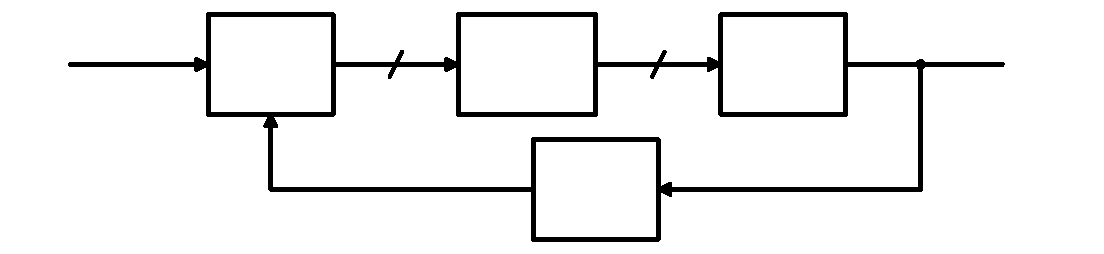
\includegraphics[scale=0.70000]{./figs/basic_adpll.pdf}\\
   % translate x=368 y=488 scale 0.38
   \putbox{1.09200in}{0.82600in}{1.20}{TDC}%
   \putbox{2.63200in}{0.24500in}{1.20}{$\div$ N}%
   \putbox{0.35700in}{0.97300in}{1.20}{$\Phi_{ref}$[n]}%
   \putbox{4.09500in}{0.97300in}{1.20}{$\Phi_{out}$[n]}%
   \putbox{2.19800in}{0.82600in}{1.20}{H$_{LF}$(z)}%
   \putbox{3.47900in}{0.82600in}{1.20}{DCO}%
   \putbox{1.67300in}{0.39200in}{1.20}{$\Phi_{div}$[n]}%
   \putbox{1.64500in}{1.02900in}{1.20}{e$_{\Phi}$[n]}%
   \putbox{2.92600in}{1.02900in}{1.20}{u[n]}%
   } % close 'parbox'
   } % close 'scalebox'
   \vspace{-\baselineskip} % this is not necessary, but looks better
\fontfamily{\rmdefault}\selectfont

	\caption{Basic ADPLL.}
	\label{fig:basic_adpll}
\end{figure}
\FloatBarrier
A basic architecture for implementing an all digital PLL is shown in figure \ref{fig:basic_adpll}, based from \cite{hsu_straayer_perrott_2008}\cite{temporiti_2009}, which replaces the phase detector of continuous PLL in figure \ref{fig:basic_pll} with a time to digital converter (TDC). Furthermore, the loop filter $\mathrm{H}_{LF}(s)$ is replaced with a discrete-time loop filter $\mathrm{H}_{LF}(z)$, and the VCO with a digitally controlled oscillator (DCO). In this architecture, all components are fully or partially digital in implementation. 

\subsubsection{Divider}\label{div_theory}
	A digital phase divider (also called frequency divider) is commonly implemented with a modulo-N counter which counts oscillator cycles \cite{weste_harris_2011}. With a divider ratio N, the output of the divider will have an active edge transition (considered to be rising edge as shown in figure \ref{fig:digital_div}) every N input cycles. Phase information is inferred from the output edge timing, which occurs with time interval N$/f_{osc}$, and is equal to the point at which output phase equals a multiple of $2\pi$. Thus a digital divider does not provider continuous phase information, but rather a sampled phase signal with rate $f_{osc}/$N. 
	\begin{figure}[htb!]
		\center\fontfamily{\sfdefault}\selectfont
% XCircuit output "digital_div.tex" for LaTeX input from digital_div.ps
\def\putbox#1#2#3#4{\makebox[0.00000in][l]{\makebox[#1][l]{}\raisebox{\baselineskip}[0.00000in][0.00000in]{\raisebox{#2}[0.00000in][0.00000in]{\scalebox{#3}{#4}}}}}
\def\rightbox#1{\makebox[0.00000in][r]{#1}}
\def\centbox#1{\makebox[0.00000in]{#1}}
\def\topbox#1{\raisebox{-0.60\baselineskip}[0.00000in][0.00000in]{#1}}
\def\midbox#1{\raisebox{-0.20\baselineskip}[0.00000in][0.00000in]{#1}}
   \scalebox{1}{
   \normalsize
   \parbox{3.15000in}{
   \includegraphics[scale=0.90000]{./figs/digital_div.pdf}\\
   % translate x=-16 y=516 scale 0.38
   \putbox{1.30500in}{0.16200in}{1.20}{$\mathrm{N}/f_{osc}$}%
   } % close 'parbox'
   } % close 'scalebox'
   \vspace{-\baselineskip} % this is not necessary, but looks better
\fontfamily{\rmdefault}\selectfont

		\caption{Digital divider signals.}
		\label{fig:digital_div}
	\end{figure}

	For PLL transfer function modeling, a digital divider behaves identically to the continuous case:
	\begin{equation}
		\Phi_{div}[n] = \frac{\Phi_{out}[n]}{\mathrm{N}}
	\end{equation}
	In the z- and s-domain the divider transfer model is:
	\begin{equation}
		\mathrm{H}_{div}(z) = \mathrm{H}_{div}(s) = \frac{\Phi_{div}(z)}{\Phi_{out}(z)} = \frac{1}{\mathrm{N}}
	\end{equation}

\subsubsection{Time to Digital Converter}
	A time to digital converter (TDC) measures the the difference $\Delta t$ in arrival of two input signal \cite{machado_cabral_alves_2019}, which in the ADPLL synthesizer is the differential between the divider signal $\Phi_{div}$[n] and the reference frequency signal $\Phi_{ref}$[n]. With a known reference frequency $f_{ref}$, the measured time differential $\Delta t$ corresponds to a phase difference $\Delta\Phi=2\pi f_{ref}\Delta t$, thus the TDC acts as a phase detector. Being digitized, a TDC will have limited resolution in time (phase), defined here to be M steps per reference cycle. Figure \ref{fig:tdc} shows the basic TDC phase detector model architecture. This has a minimum step size in time of $\Delta t_{step}$ = $1/Mf_{ref}$. To map the output to digitized value, the model applies a scale factor M$/2\pi$ and floor rounding, so one least significant bit (LSB) of the output $e_\Phi[n]$ equates to $\Delta t_{step}$ timing error between inputs $\Phi_{div}$[n] and $\Phi_{ref}$[n]. The described TDC model in sampled-time equation form is in equation \ref{eq:tdc_disc_time_model}.

	% It takes input phase signals $\Phi_{div}$[n] and $\Phi_{ref}$[n], and outputs a digital phase error word $e_\Phi[n]$.

	\begin{figure}[htb!]
		\center\include{./figs/tdc}
		\caption{TDC model.}
		\label{fig:tdc}
	\end{figure}
	\FloatBarrier
	\begin{equation}\label{eq:tdc_disc_time_model}
		e_\Phi[n] = \left\lfloor\frac{\mathrm{M}}{2\pi}(\Phi_{ref}[n] - \Phi_{div}[n])\right\rfloor
	\end{equation}
	The TDC z-domain representation is equation \ref{eq:tdc_z}. For purposes of PLL loop gain calculation, the TDC transfer function is in equation \ref{eq:tdc_tf}, which accounts for phase-to-digital domain conversion gain. Effects of quantization will be handled separately in section \ref{pn_theory}.
	\begin{equation}\label{eq:tdc_z}
		e_\Phi(z) = \frac{\mathrm{M}}{2\pi}(\Phi_{ref}(z) - \Phi_{div}(z))
	\end{equation}	
	\begin{equation}\label{eq:tdc_tf}
		\mathrm{H}_{TDC}(z) = \mathrm{H}_{TDC}(s) = \frac{\mathrm{M}}{2\pi}
	\end{equation}	
	\FloatBarrier

\subsubsection{Discrete Time Loop Filter}\label{lf-discretization}
	The discrete-time loop filter design will be derived from the continuous canonical loop filter (equation \ref{eq:lf_general_form}) via application of a s-to-z domain transformation. The bilinear transform \cite{proakis_1993_bilinear} allows for such conversion from continuous transfer function to discrete representation. In the case presented in this work, the loop filter sampling rate $f_s$=$f_{ref}$ is constrained to be much greater than the PLL loop bandwidth ($f_s > 10\cdot\mathrm{BW}_{loop}$). Thus, a simpler transformation is permissible, derived through Taylor series approximation of the definition of complex variable z=$re^{s\Delta T}$ \cite{proakis_1993_z} for values on the unit circle, i.e. r=1. This will be referred to as the approximate bilinear transform in this work. Given the $1/\Delta T_s$=$f_{s}$ as the relation for sampling rate, then:
	\begin{align*}
		z^{-1} &= e^{-s\Delta T_s} && \text{(definition of z on unit circle)} \\
		&= \sum_{k=0}^\infty\frac{(-s\Delta T_s)^k}{k!} && \text{(exponential Taylor series)} \\
		&\approx 1-s\Delta T_s &&\text{(if $|s\Delta T_s| = 2\pi\mathrm{BW}_{loop}\cdot \Delta T_s << 1$)} \\
	\end{align*}
	Thus the s-to-z and z-to-s identities for the approximated bilinear transform are:
	\begin{align}
		z^{-1} &= 1-s\Delta T_s\\
		s &= \frac{1}{\Delta T_s}(1-z^{-1}) \label{eq:s_to_z_xfrm}
	\end{align}
	Applying equation \ref{eq:s_to_z_xfrm} to the general loop filter of equation \ref{eq:lf_general_form} yields the z-domain loop filter:
	\begin{align}
		\textnormal{H}_{LF}(z) &= \left.\textnormal{H}_{LF}(s)\right\vert_{s=\frac{1}{\Delta T_s}(1-z^{-1})} = \left.\frac{\sum_{j=0}^Z b_js^j}{\sum_{k=0}^P a_ks^k}\right\vert_{s=\frac{1}{\Delta T_s}(1-z^{-1})}\\
		&= \frac{\sum_{j=0}^Z \frac{b_j}{\Delta T_s^j}(1-z^{-1})^j}{\sum_{k=0}^P \frac{a_k}{\Delta T_k}(1-z^{-1})^k} \label{eq:z_general_lf}
	\end{align}
	Equation \ref{eq:z_general_lf} is transformed into a digitally implementable form by reorganizing into the canonical representation of equation \ref{eq:canonical_z_tf}, which then determines the tap coefficients for the sampled-time difference equation in equation \ref{eq:cananical_diff_eq}. 
	\begin{align}
		\textnormal{H}_{LF}(z) &= \frac{\sum_{j=0}^P b_j^{'}z^{-j}}{1+\sum_{k=1}^Z a_k^{'}z^{-k}}\label{eq:canonical_z_tf} \\
		y[n]&= -\sum_{k=1}^P a_k^{'}y[n-k] + \sum_{j=0}^Z b_j^{'}x[n-j] \label{eq:cananical_diff_eq}
	\end{align}
	The obtained difference equation is directly implementable in digital hardware with a direct form-I IIR filter \cite{proakis_1993} shown in figure \ref{fig:filt_implementation}. The filter coefficients $\{a_1^{'}, ..., a_P^{'}\}$ and $\{b_0^{'}, ..., b_Z^{'}\}$ must be quantized into finite resolution fixed point words for a complete digital implementation. The delay elements ($z^{-1}$ blocks) are implementable digitally as registers, the coefficient gains are implementable with array multipliers, and the adders are implementable with digital adders. Effects of quantization will be discussed in section \ref{pn_theory}.
	\begin{figure}[htb!]
		\center\include{./figs/direct_type_1_primed}
		\caption{Direct form I implementation of IIR filter.}
		\label{fig:filt_implementation}
	\end{figure}


\subsubsection{Digitally Controlled Oscillator}
	The digitally controlled oscillator (DCO) varies from a VCO by only accepting a digital frequency tuning signal, called the oscillator tuning word (OTW). A DCO is modeled in discrete time as a recursive phase integrator, dependent on (a) the DCO gain $K_{DCO}$, equal to the frequency tuning of the oscillator per LSB of the OTW, (b) the current state of the OTW u[n], and (c) the PLL sampling period $\Delta T_s$=$f_{ref}^{-1}$.
	\begin{equation}
		\Phi_{out}[n] = \Phi_{out}[n-1] + 2\pi K_{DCO}u[n]\Delta T_s
	\end{equation}
	Application of the z-transform yields equation \ref{eq:hdcoz}, and successive application of the bilinear transform to the DCO transfer function yields the continuous approximation of equation \ref{eq:hdcos}.
	\begin{equation}\label{eq:hdcoz}
		\mathrm{H}_{DCO}(z) = \frac{\Phi_{out}(z)}{u(z)} = \frac{2\pi K_{DCO}\Delta T_s}{1-z^{-1}}
	\end{equation}
	\begin{equation}\label{eq:hdcos}
		\mathrm{H}_{DCO}(s) = \frac{\Phi_{out}(s)}{u(s)} = \frac{2\pi K_{DCO}\Delta T_s}{1-(1-s\Delta T_s)} = \frac{2\pi K_{DCO}}{s} 
	\end{equation}

\subsubsection{Discrete Time PLL Transfer Function}\label{discrete_pll_tf}
	\begin{figure}[htb!]
		\center\fontfamily{\sfdefault}\selectfont
% XCircuit output "discrete_pll.tex" for LaTeX input from discrete_pll.ps
\def\putbox#1#2#3#4{\makebox[0.00000in][l]{\makebox[#1][l]{}\raisebox{\baselineskip}[0.00000in][0.00000in]{\raisebox{#2}[0.00000in][0.00000in]{\scalebox{#3}{#4}}}}}
\def\rightbox#1{\makebox[0.00000in][r]{#1}}
\def\centbox#1{\makebox[0.00000in]{#1}}
\def\topbox#1{\raisebox{-0.60\baselineskip}[0.00000in][0.00000in]{#1}}
\def\midbox#1{\raisebox{-0.20\baselineskip}[0.00000in][0.00000in]{#1}}
   \scalebox{1}{
   \normalsize
   \parbox{6.53333in}{
   \includegraphics[scale=0.70000]{./figs/discrete_pll.pdf}\\
   % translate x=416 y=508 scale 0.38
   \putbox{0.39200in}{1.04300in}{1.20}{$\Phi_{ref}$[n]}%
   \putbox{1.82000in}{0.46200in}{1.20}{$\Phi_{div}$[n]}%
   \putbox{2.65300in}{1.07800in}{1.20}{e$_\Phi$[n]}%
   \putbox{1.71500in}{1.12000in}{1.20}{\rotatebox{-360}{$\frac{\mathrm{M}}{2\pi}$}}%
   \putbox{1.40700in}{1.04300in}{1.20}{$\Phi_e$}%
   \putbox{2.13500in}{0.91700in}{1.20}{$\lfloor x\rfloor$}%
   \putbox{0.97300in}{1.36500in}{0.90}{TDC}%
   \putbox{3.20600in}{0.91700in}{1.20}{H$_{LF}$(z)}%
   \putbox{3.93400in}{1.07800in}{1.20}{u[n]}%
   \putbox{4.38200in}{0.93100in}{1.20}{$\frac{2\pi K_{DCO}T}{1-z^{-1}}$}%
   \putbox{5.20100in}{1.04300in}{1.20}{$\Phi_{out}$[n]}%
   \putbox{3.27600in}{0.32900in}{1.20}{$\div$ N}%
   \putbox{4.35400in}{1.23200in}{0.90}{DCO}%
   } % close 'parbox'
   } % close 'scalebox'
   \vspace{-\baselineskip} % this is not necessary, but looks better
\fontfamily{\rmdefault}\selectfont

		\caption{Discrete time PLL model.}
		\label{fig:discrete_pll2}
	\end{figure}
	The transfer function for the full discrete-time PLL of figure \ref{fig:discrete_pll2} can be computed in the z-domain, and also approximated continuously. The open loop z-domain transfer function is:
	\begin{align}
		\mathrm{L}(z) &= \mathrm{H}_{TDC}(z)\mathrm{H}_{LF}(z)\mathrm{H}_{DCO}(z)\mathrm{H}_{DIV}(z)
		= \frac{\mathrm{M}}{\mathrm{N}}\frac{K_{DCO}\Delta T_s}{(1-z^{-1})}\frac{\sum_{j=0}^Z b_j(1-z^{-1})^j}{\sum_{k=0}^P a_k(1-z^{-1})^k}\label{eq:z_open_loop}
	\end{align}
	The closed loop z-domain PLL phase transfer function is:
	\begin{align}
		\mathrm{T}(z) = \frac{\Phi_{out}(z)}{\Phi_{ref}(z)} &= \frac{\mathrm{M}K_{DCO}\Delta T_s\sum_{j=0}^Z b_j(1-z^{-1})^j}{\sum_{k=0}^P a_k(1-z^{-1})^{k+1} + K_{DCO}\Delta T_s\frac{\mathrm{M}}{\mathrm{N}}\sum_{j=0}^Z b_j(1-z^{-1})^j}%\\
		%&= \mathrm{N}\frac{\mathrm{L}(z)}{1+\mathrm{L}(z)}\\
	\end{align}
	The s-domain approximation of the transfer function is:
	\begin{align}
		\mathrm{L}(s) = \mathrm{H}_{TDC}(s)\mathrm{H}_{LF}(s)\mathrm{H}_{DCO}(s)\mathrm{H}_{DIV}(s) = \frac{\mathrm{M}}{\mathrm{N}}\frac{K_{DCO}}{s} \frac{\sum_{j=0}^Z b_js^j}{\sum_{k=0}^P a_ks^k}
	\end{align}
	And in closed loop configuration the s-domain PLL phase transfer function is:
	\begin{align}
		\mathrm{T}(s)=\frac{\Phi_{out}(s)}{\Phi_{ref}(s)} = \frac{\mathrm{M}K_{DCO}\sum_{j=0}^Z b_js^j}{\sum_{k=0}^P a_ks^{k+1} + \frac{\mathrm{M}}{\mathrm{N}}K_{DCO}\sum_{j=0}^Z b_js^j} = \mathrm{N}\frac{\mathrm{L}(s)}{1+\mathrm{L}(s)}
	\end{align}

%%%%%%%%%%%%%%%%%%%%%%%%%%%%%%%%%%%%%%%%%%%%%%%%%%%%%%%%%%%%%%%%%%%%%%%%%%%%%%%%
%%%%%%%%%%%%%%%%%%%%%%%%%%%%%%%%%%%%%%%%%%%%%%%%%%%%%%%%%%%%%%%%%%%%%%%%%%%%%%%%
% Noise
%%%%%%%%%%%%%%%%%%%%%%%%%%%%%%%%%%%%%%%%%%%%%%%%%%%%%%%%%%%%%%%%%%%%%%%%%%%%%%%%
%%%%%%%%%%%%%%%%%%%%%%%%%%%%%%%%%%%%%%%%%%%%%%%%%%%%%%%%%%%%%%%%%%%%%%%%%%%%%%%%

\subsection{ADPLL Noise Model} \label{pn_theory}
The noise in the discrete-time ADPLL results from quantization and from stochastic sources. Quantization results from round off errors introduced in the digitization of PLL components (in the TDC, loop filter, and DCO). Stochastic noise results from thermal and flicker noise in the PLL components when considered in an analog viewpoint (present in the DCO, divider and TDC). The noise generated by these quantization sources will be discussed in the following sections.% based on a modeling and noise analysis approach from \cite{perrott_2002}.

\subsubsection{TDC Noise}\label{tdc_noise}
	The predominant noise source of within a TDC is due to quantization. This source will dominate overall noise within a PLL's closed loop bandwidth \cite{shen_2014}\cite{takinami_2011}\cite{lu_andreani_2010}, so its consideration is critical for PLL performance. As will be seen, a straightforward approach to model quantization noise is to treat it as an additive signal component as shown in figure \ref{fig:tdc_add_pn}.
	\begin{figure}[htb!]
	    \centering
	    \begin{subfigure}{0.5\textwidth}
	        \centering
	        \include{./figs/tdc}
	        \caption{ }
	        \label{fig:tdc1}
	    \end{subfigure}%
	    \begin{subfigure}{0.5\textwidth}
	        \centering
	        \fontfamily{\sfdefault}\selectfont
% XCircuit output "tdc_quant.tex" for LaTeX input from tdc_quant.ps
\def\putbox#1#2#3#4{\makebox[0.00000in][l]{\makebox[#1][l]{}\raisebox{\baselineskip}[0.00000in][0.00000in]{\raisebox{#2}[0.00000in][0.00000in]{\scalebox{#3}{#4}}}}}
\def\rightbox#1{\makebox[0.00000in][r]{#1}}
\def\centbox#1{\makebox[0.00000in]{#1}}
\def\topbox#1{\raisebox{-0.60\baselineskip}[0.00000in][0.00000in]{#1}}
\def\midbox#1{\raisebox{-0.20\baselineskip}[0.00000in][0.00000in]{#1}}
   \scalebox{1}{
   \normalsize
   \parbox{3.50000in}{
   \includegraphics[scale=0.70000]{./figs/tdc_quant.pdf}\\
   % translate x=432 y=396 scale 0.38
   \putbox{0.46200in}{0.63700in}{1.20}{$\Phi_{ref}$[n]}%
   \putbox{1.35100in}{0.08400in}{1.20}{$\Phi_{div}$[n]}%
   \putbox{2.68100in}{0.66500in}{1.20}{e$_\Phi$[n]}%
   \putbox{1.77800in}{0.70700in}{1.20}{\rotatebox{-360}{$\frac{\mathrm{M}}{2\pi}$}}%
   \putbox{1.47000in}{0.63700in}{1.20}{$\Phi_e$}%
   \putbox{2.31700in}{0.97300in}{1.20}{q$_{TDC}$[n]}%
   \putbox{1.02900in}{0.95900in}{1.20}{TDC}%
   } % close 'parbox'
   } % close 'scalebox'
   \vspace{-\baselineskip} % this is not necessary, but looks better
\fontfamily{\rmdefault}\selectfont

	        \caption{ }
	        \label{fig:tdc_add_pn}
	    \end{subfigure}
	    % \caption{Approximate model for ring oscillator inverter delay cell.}
	    \label{fig:tdc_pn_model}
	    \caption{\textbf{(a)} TDC Model, \textbf{(b)} TDC additive noise model.}
	\end{figure}
	\FloatBarrier
	Suppose the quantized signal $e_\Phi$[n] out of the TDC can be represented as the sum of its unquantized representation $\Phi_e\frac{\mathrm{M}}{2\pi}$ with a quantization error signal $\mathrm{q}_{TDC}[n]$, as in figure \ref{fig:quantization}.
	\begin{figure}[htb!]
		\center\fontfamily{\sfdefault}\selectfont
% XCircuit output "quantization.tex" for LaTeX input from quantization.ps
\def\putbox#1#2#3#4{\makebox[0.00000in][l]{\makebox[#1][l]{}\raisebox{\baselineskip}[0.00000in][0.00000in]{\raisebox{#2}[0.00000in][0.00000in]{\scalebox{#3}{#4}}}}}
\def\rightbox#1{\makebox[0.00000in][r]{#1}}
\def\centbox#1{\makebox[0.00000in]{#1}}
\def\topbox#1{\raisebox{-0.60\baselineskip}[0.00000in][0.00000in]{#1}}
\def\midbox#1{\raisebox{-0.20\baselineskip}[0.00000in][0.00000in]{#1}}
   \scalebox{1}{
   \normalsize
   \parbox{4.24010in}{
   \includegraphics[scale=0.70000]{./figs/quantization.pdf}\\
   % translate x=304 y=240 scale 0.38
   \putbox{0.04200in}{1.09200in}{0.96}{$e_\Phi$[n]}%
   \putbox{1.32300in}{0.04200in}{0.96}{t=nT}%
   \putbox{1.32300in}{1.09200in}{0.96}{$\frac{\mathrm{M}}{2\pi}\Phi_e$[n]}%
   \putbox{2.77900in}{0.04200in}{0.96}{\rotatebox{-360}{t}}%
   \putbox{4.24200in}{0.50400in}{0.96}{t}%
   \putbox{2.72300in}{1.09200in}{0.96}{q$_{\mathrm{TDC}}$[n]}%
   \putbox{3.47900in}{0.85400in}{0.96}{$+\Delta/2$}%
   \putbox{3.47900in}{0.44800in}{0.96}{$-\Delta/2$}%
   } % close 'parbox'
   } % close 'scalebox'
   \vspace{-\baselineskip} % this is not necessary, but looks better
\fontfamily{\rmdefault}\selectfont

		\caption{Quantization as via additive error signal.}
		\label{fig:quantization}
	\end{figure}
	\FloatBarrier
	Based on \cite{widrow_1961}, if the quantization noise signal $\mathrm{q}_{TDC}[n]$ is uncorrelated to unquantized signal $\Phi_e\frac{\mathrm{M}}{2\pi}$, it has the statistical property that it is uniformly distributed in the range $[-\Delta/2, \Delta/2]$, i.e. $P_q(Q=q) =\mathrm{U}(-\Delta/2, \Delta/2)$. $\Delta$ is the quantization step size. The variance, or power, of the TDC quantization noise signal is:
	\begin{equation}\label{eq:tdc_noise}
		\sigma_{q_{TDC}}^2 = \int_{-\infty}^\infty q^2P_q(Q=q)dq =  \int_{-\Delta/2}^{\Delta/2}\frac{q^2}{\Delta}dq = \frac{\Delta^2}{12}
	\end{equation}
	Since $e_\Phi$[n] is a digital signal, the quantization step size is $\Delta$=1 LSB. The TDC quantization noise power is therefore $\sigma_{q_{TDC}}^2 = 1/12$ LSB$^2$. If the quantization noise is presumed to be white, and the TDC sampling rate is $f_{ref}$, the quantization noise power spectral density (PSD) is then given in equation \ref{eq:tdc_quant_psd}. 
	\begin{equation}\label{eq:tdc_quant_psd}
		S_{qn_{TDC}}(f) = \frac{P_{q_{TDC}}}{\Delta f} = \frac{\sigma_{q_{TDC}}^2}{f_{ref}} = \frac{\Delta^2}{12f_{ref}} = \frac{1}{12f_{ref}} \hspace{1em}\frac{[\text{LSB}]^2}{[\text{Hz}]}
	\end{equation}

\subsubsection{DCO Noise}\label{dco_noise}
	Noise in a DCO is resulting from (a) quantization of the oscillator tuning word u[n], and (b) from thermal and stochastic sources. In the digital PLL, the OTW quantization occurs in the loop filter, so this will be analyzed in the later loop filter section (\ref{lf_noise}). Thus oscillator thermal/stochastic noise will be considered, based on Leeson's model for oscillator phase noise \cite{leeson_1966}. Leeson's model considers noise power density at an offset $\Delta f$ from the oscillator tone (carrier). Noise power density is represented with the function $\mathcal{L}(\Delta f)$, which is the noise power density normalized to the power of the oscillator carrier tone, in other words in units of dBc/Hz. Leeson's model divides phase noise into three regions, illustrated in figure \ref{fig:leeson_pn}: (1) flicker-noise dominated, with a slope of -30 dB/decade, (2) white frequency-noise dominated, with -20 dB per decade, and (3) a flat region, limited by the thermal noise floor or amplitude noise. It is noted that phase noise components are at frequencies different than the carrier, hence are orthogonal, and can be treated as independent components that are added to the main oscillator tone signal for analysis. Figure \ref{fig:dco_noise} demonstrates the application of this principle for modeling of the DCO phase noise $\Phi_{n_{DCO}}$ as an additive process to the oscillator phase $\Phi_{osc}$, thus $\Phi_{out}$ = $\Phi_{osc}$ + $\Phi_{n_{DCO}}$.


	\begin{figure}[htb!]
	    \centering
	    \begin{subfigure}{0.45\textwidth}
	        \centering
			\fontfamily{\sfdefault}\selectfont
% XCircuit output "leeson_pn.tex" for LaTeX input from leeson_pn.ps
\def\putbox#1#2#3#4{\makebox[0.00000in][l]{\makebox[#1][l]{}\raisebox{\baselineskip}[0.00000in][0.00000in]{\raisebox{#2}[0.00000in][0.00000in]{\scalebox{#3}{#4}}}}}
\def\rightbox#1{\makebox[0.00000in][r]{#1}}
\def\centbox#1{\makebox[0.00000in]{#1}}
\def\topbox#1{\raisebox{-0.60\baselineskip}[0.00000in][0.00000in]{#1}}
\def\midbox#1{\raisebox{-0.20\baselineskip}[0.00000in][0.00000in]{#1}}
   \scalebox{1}{
   \normalsize
   \parbox{2.68750in}{
   \includegraphics[scale=0.80000]{./figs/leeson_pn.pdf}\\
   % translate x=-248 y=245 scale 0.38
   \putbox{1.88000in}{0.06400in}{0.90}{$\log(\Delta f)$}%
   \putbox{0.80800in}{1.23200in}{0.72}{-30 dB/dec}%
   \putbox{0.80800in}{1.09600in}{0.72}{$\propto f^{-3}$}%
   \putbox{1.34400in}{0.73600in}{0.72}{$\propto f^{-2}$}%
   \putbox{1.34400in}{0.86400in}{0.72}{-20 dB/dec}%
   \putbox{0.80800in}{0.13600in}{0.72}{\rotatebox{-360}{$f_1$}}%
   \putbox{1.60800in}{0.13600in}{0.72}{\rotatebox{-360}{$f_2$}}%
   \putbox{0.04800in}{1.40000in}{0.90}{$\mathcal{L}(\Delta f)$}%
   } % close 'parbox'
   } % close 'scalebox'
   \vspace{-\baselineskip} % this is not necessary, but looks better
\fontfamily{\rmdefault}\selectfont

			\caption{ }
			\label{fig:leeson_pn}
	    \end{subfigure}
	    \begin{subfigure}{0.5\textwidth}
	        \centering
			\fontfamily{\sfdefault}\selectfont
% XCircuit output "dco_noise.tex" for LaTeX input from dco_noise.ps
\def\putbox#1#2#3#4{\makebox[0.00000in][l]{\makebox[#1][l]{}\raisebox{\baselineskip}[0.00000in][0.00000in]{\raisebox{#2}[0.00000in][0.00000in]{\scalebox{#3}{#4}}}}}
\def\rightbox#1{\makebox[0.00000in][r]{#1}}
\def\centbox#1{\makebox[0.00000in]{#1}}
\def\topbox#1{\raisebox{-0.60\baselineskip}[0.00000in][0.00000in]{#1}}
\def\midbox#1{\raisebox{-0.20\baselineskip}[0.00000in][0.00000in]{#1}}
   \scalebox{1}{
   \normalsize
   \parbox{3.56562in}{
   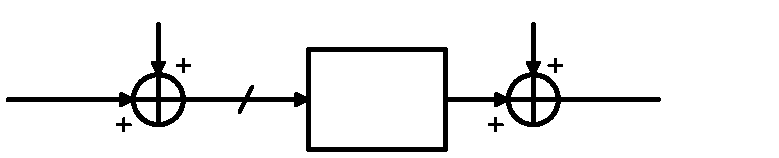
\includegraphics[scale=0.70000]{./figs/dco_noise.pdf}\\
   % translate x=-384 y=320 scale 0.38
   \putbox{1.02900in}{0.39200in}{0.96}{u[n]}%
   \putbox{1.48400in}{0.24500in}{0.96}{$\frac{2\pi K_{DCO}T}{1-z^{-1}}$}%
   \putbox{2.66700in}{0.34300in}{0.96}{$\Phi_{out}$[n]}%
   \putbox{0.78400in}{0.60900in}{0.96}{q$_{OTW}$[n]}%
   \putbox{0.18200in}{0.37800in}{0.96}{$\hat{\textnormal{u}}$[n]}%
   \putbox{2.54800in}{0.62300in}{0.96}{$\Phi_{n_{DCO}}$[n]}%
   } % close 'parbox'
   } % close 'scalebox'
   \vspace{-\baselineskip} % this is not necessary, but looks better
\fontfamily{\rmdefault}\selectfont

			\caption{ }
			\label{fig:dco_noise}
	    \end{subfigure}%
	    % \caption{Approximate model for ring oscillator inverter delay cell.}
	    \label{fig:osc_pn_figs}
	    \caption{\textbf{(a)} Leeson model for phase noise, \textbf{(b)} DCO additive noise model.}
	\end{figure}
	\FloatBarrier
	The equation for $\mathcal{L}(\Delta f)$ (from \cite{lee_hajimiri_2000}) is in equation \ref{eq:leesons}, and is dependent on temperature T, excess noise factor F, oscillator power P, oscillator Q factor, and the transition frequencies $f_1$ and $f_2$ that separate the different noise regions. It is of interest to note that the phase noise relative to the carrier will increase as power decreases, which provides challenge for creating low power oscillators with acceptable phase noise characteristics.
	\begin{equation}\label{eq:leesons}
	\mathcal{L}(\Delta f) = 10\log_{10}\left[\frac{2\text{F}k_B\text{T}}{\text{P}}\left(1+\left(\frac{f_2}{2Q\Delta f}\right)^2\right)\left(1+\frac{f_1}{|\Delta f|}\right)\right] = S_{\Phi n_{DCO}}(\Delta f)
	\end{equation}
	For notational consistency, the following redefinition is used in the remainder of this paper: $S_{\Phi n_{DCO}}(f) = \mathcal{L}(\Delta f)|_{\Delta f = f}$

\subsubsection{Divider Noise}
	\begin{figure}[htb!]
	    \centering
	    \begin{subfigure}{0.5\textwidth}
	        \centering
	        \fontfamily{\sfdefault}\selectfont
% XCircuit output "div_noise_model.tex" for LaTeX input from div_noise_model.ps
\def\putbox#1#2#3#4{\makebox[0.00000in][l]{\makebox[#1][l]{}\raisebox{\baselineskip}[0.00000in][0.00000in]{\raisebox{#2}[0.00000in][0.00000in]{\scalebox{#3}{#4}}}}}
\def\rightbox#1{\makebox[0.00000in][r]{#1}}
\def\centbox#1{\makebox[0.00000in]{#1}}
\def\topbox#1{\raisebox{-0.60\baselineskip}[0.00000in][0.00000in]{#1}}
\def\midbox#1{\raisebox{-0.20\baselineskip}[0.00000in][0.00000in]{#1}}
   \scalebox{1}{
   \normalsize
   \parbox{2.75260in}{
   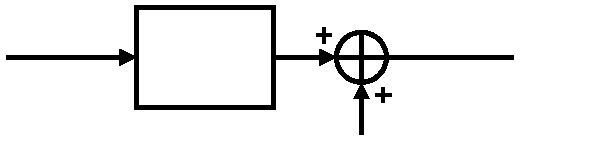
\includegraphics[scale=0.70000]{./figs/div_noise_model.pdf}\\
   % translate x=-96 y=524 scale 0.38
   \putbox{0.04200in}{0.53200in}{1.20}{$\Phi_{out}$[n]}%
   \putbox{0.79800in}{0.39200in}{1.20}{$\div \mathrm{N}$}%
   \putbox{1.74300in}{0.05600in}{1.20}{$\Phi_{n_{div}}$}%
   \putbox{1.84800in}{0.53200in}{1.20}{$\Phi_{div}$[n]}%
   } % close 'parbox'
   } % close 'scalebox'
   \vspace{-\baselineskip} % this is not necessary, but looks better
\fontfamily{\rmdefault}\selectfont

	        \caption{ }
	        \label{fig:div_pn_model}
	    \end{subfigure}%
	    \begin{subfigure}{0.5\textwidth}
	        \centering
	        \fontfamily{\sfdefault}\selectfont
% XCircuit output "div_jitter.tex" for LaTeX input from div_jitter.ps
\def\putbox#1#2#3#4{\makebox[0.00000in][l]{\makebox[#1][l]{}\raisebox{\baselineskip}[0.00000in][0.00000in]{\raisebox{#2}[0.00000in][0.00000in]{\scalebox{#3}{#4}}}}}
\def\rightbox#1{\makebox[0.00000in][r]{#1}}
\def\centbox#1{\makebox[0.00000in]{#1}}
\def\topbox#1{\raisebox{-0.60\baselineskip}[0.00000in][0.00000in]{#1}}
\def\midbox#1{\raisebox{-0.20\baselineskip}[0.00000in][0.00000in]{#1}}
   \scalebox{1}{
   \normalsize
   \parbox{2.61563in}{
   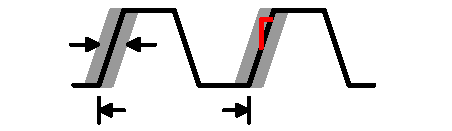
\includegraphics[scale=0.90000]{./figs/div_jitter.pdf}\\
   % translate x=-116 y=432 scale 0.38
   \putbox{0.80100in}{0.07200in}{1.20}{$\mathrm{N}/f_{osc}$}%
   \putbox{0.05400in}{0.61200in}{1.20}{$\sigma_{\Phi n_{div}}$}%
   \putbox{1.28700in}{0.59400in}{1.20}{$\frac{dV}{dt}$}%
   } % close 'parbox'
   } % close 'scalebox'
   \vspace{-\baselineskip} % this is not necessary, but looks better
\fontfamily{\rmdefault}\selectfont

	        \caption{ }
	        \label{fig:div_jitter}
	    \end{subfigure}
	    % \caption{Approximate model for ring oscillator inverter delay cell.}
	    \label{fig:div_pn}
	    \caption{\textbf{(a)} Divider noise model, \textbf{(b)} Digital divider output jitter.}
	\end{figure}
	\FloatBarrier
	Divider noise is manifested as jitter (with RMS distribution in time of $\sigma_{t n_{div}}$) on the divider output. If the divider is a digital circuit, with edge rate $dV/dt$, and subject to thermal noise in the form of an additive voltage $v_n$, with noise power of $\sigma_{v_n}^2$, the divider phase noise power added to the divider output is:
	\begin{equation}
		\sigma_{\Phi n_{div}}^2 = \omega^2_{ref}\sigma^2_{t n_{div}}  =\omega^2_{ref}\left(\frac{dV}{dt}\right)^{-2}\sigma_{v_n}^2
	\end{equation}
	At lock, the output of a digital divider will have an update rate $f_{{osc}}/\mathrm{N} \approx f_{ref}$, which can be treated as the sampling rate of the output phase signal $\Phi_{div}[n]$ as mentioned in section \ref{div_theory}. If the divider phase noise power is confined into a bandwidth equal to the PLL reference frequency $f_{ref}$, the spectral density of divider noise is:
	\begin{equation}
		S_{\Phi n_{div}}(f) = \frac{\sigma_{\Phi n_{div}}^2}{f_{ref}} = 2\pi\omega_{ref}\sigma^2_{t n_{div}}  =2\pi\omega_{ref}\left(\frac{dV}{dt}\right)^{-2}\sigma_{v_n}^2\hspace{1em}\frac{[\text{rad}]^2}{[\text{Hz}]}
	\end{equation}

\subsubsection{Loop Filter Noise - Direct Form I}\label{lf_noise}
	In a digital loop filter, quantization noise arises from rounding errors due to finite precision in the digital arithmetic circuits that implement the filter \cite{proakis_1993_fwe}. Quantization noise power here will be derived under the assumption of a direct form I structure implementating the filter, with B bits in each fixed point data word throughout the digital loop filter. In a digital implementation of the canonical z-domain transfer function in equation \ref{eq:canon_z_tf} as the direct form I structure of figure \ref{fig:direct_type_1_ideal}, delays are constructed using registers, adders with digital adders, and the filter coefficient gain terms $\{a_1, ... a_N; b_0, ..., b_M\}$ with digital multipliers. The registers and adders do not introduce extra round-off error beyond that already existing (if overflows do not occur). However, the multipliers will if the products resulting from two B bit words (nominally 2B bits), are mapped back onto B bit words.
	\begin{equation}
		\textnormal{H}_{LF}(z) = \frac{\sum_{j=0}^Z b_jz^{-j}}{1+\sum_{k=1}^P a_kz^{-k}}\label{eq:canon_z_tf}
	\end{equation}
	\FloatBarrier
	Quantization in this case can be represented by adding a quantization error signal $q_x$[n] to the result of each ideal multiplication, as shown in figure \ref{fig:direct_type_1_quant}. This is the same approach for TDC quantization noise in section \ref{tdc_noise}. The noise power associated with each q$_x$[n] is identical, with $\sigma_{qx}^2 = 1/12$ LSB$^2$. 

	\begin{figure}[htb!]
	    \centering
	    \begin{subfigure}{0.5\textwidth}
	        \centering
	        \fontfamily{\sfdefault}\selectfont
% XCircuit output "direct_type_1.tex" for LaTeX input from direct_type_1.ps
\def\putbox#1#2#3#4{\makebox[0.00000in][l]{\makebox[#1][l]{}\raisebox{\baselineskip}[0.00000in][0.00000in]{\raisebox{#2}[0.00000in][0.00000in]{\scalebox{#3}{#4}}}}}
\def\rightbox#1{\makebox[0.00000in][r]{#1}}
\def\centbox#1{\makebox[0.00000in]{#1}}
\def\topbox#1{\raisebox{-0.60\baselineskip}[0.00000in][0.00000in]{#1}}
\def\midbox#1{\raisebox{-0.20\baselineskip}[0.00000in][0.00000in]{#1}}
   \scalebox{1}{
   \normalsize
   \parbox{2.59948in}{
   \includegraphics[scale=0.70000]{./figs/direct_type_1.pdf}\\
   % translate x=936 y=992 scale 0.38
   \putbox{0.04200in}{1.42800in}{0.96}{x[n]}%
   \putbox{2.28200in}{1.33700in}{0.96}{y[n]}%
   \putbox{0.37800in}{1.07800in}{0.96}{$z^{-1}$}%
   \putbox{0.84000in}{1.45600in}{0.96}{b$_0$}%
   \putbox{0.84000in}{0.98700in}{0.96}{b$_1$}%
   \putbox{2.12800in}{1.07800in}{0.96}{$z^{-1}$}%
   \putbox{2.12800in}{0.34300in}{0.96}{$z^{-1}$}%
   \putbox{1.71500in}{1.00100in}{0.96}{-a$_1$}%
   \putbox{1.70100in}{0.27300in}{0.96}{-a$_\mathrm{P}$}%
   \putbox{2.28200in}{0.86800in}{0.96}{y[n-1]}%
   \putbox{0.37800in}{0.34300in}{0.96}{$z^{-1}$}%
   \putbox{0.84000in}{0.25900in}{0.96}{b$_\mathrm{Z}$}%
   } % close 'parbox'
   } % close 'scalebox'
   \vspace{-\baselineskip} % this is not necessary, but looks better
\fontfamily{\rmdefault}\selectfont

	        \vspace{1.2em}
	        \caption{ }
	        \label{fig:direct_type_1_ideal}
	    \end{subfigure}%
	    \begin{subfigure}{0.5\textwidth}
	        \centering
	        \fontfamily{\sfdefault}\selectfont
% XCircuit output "direct_type_1_quant.tex" for LaTeX input from direct_type_1_quant.ps
\def\putbox#1#2#3#4{\makebox[0.00000in][l]{\makebox[#1][l]{}\raisebox{\baselineskip}[0.00000in][0.00000in]{\raisebox{#2}[0.00000in][0.00000in]{\scalebox{#3}{#4}}}}}
\def\rightbox#1{\makebox[0.00000in][r]{#1}}
\def\centbox#1{\makebox[0.00000in]{#1}}
\def\topbox#1{\raisebox{-0.60\baselineskip}[0.00000in][0.00000in]{#1}}
\def\midbox#1{\raisebox{-0.20\baselineskip}[0.00000in][0.00000in]{#1}}
   \scalebox{1}{
   \normalsize
   \parbox{2.92760in}{
   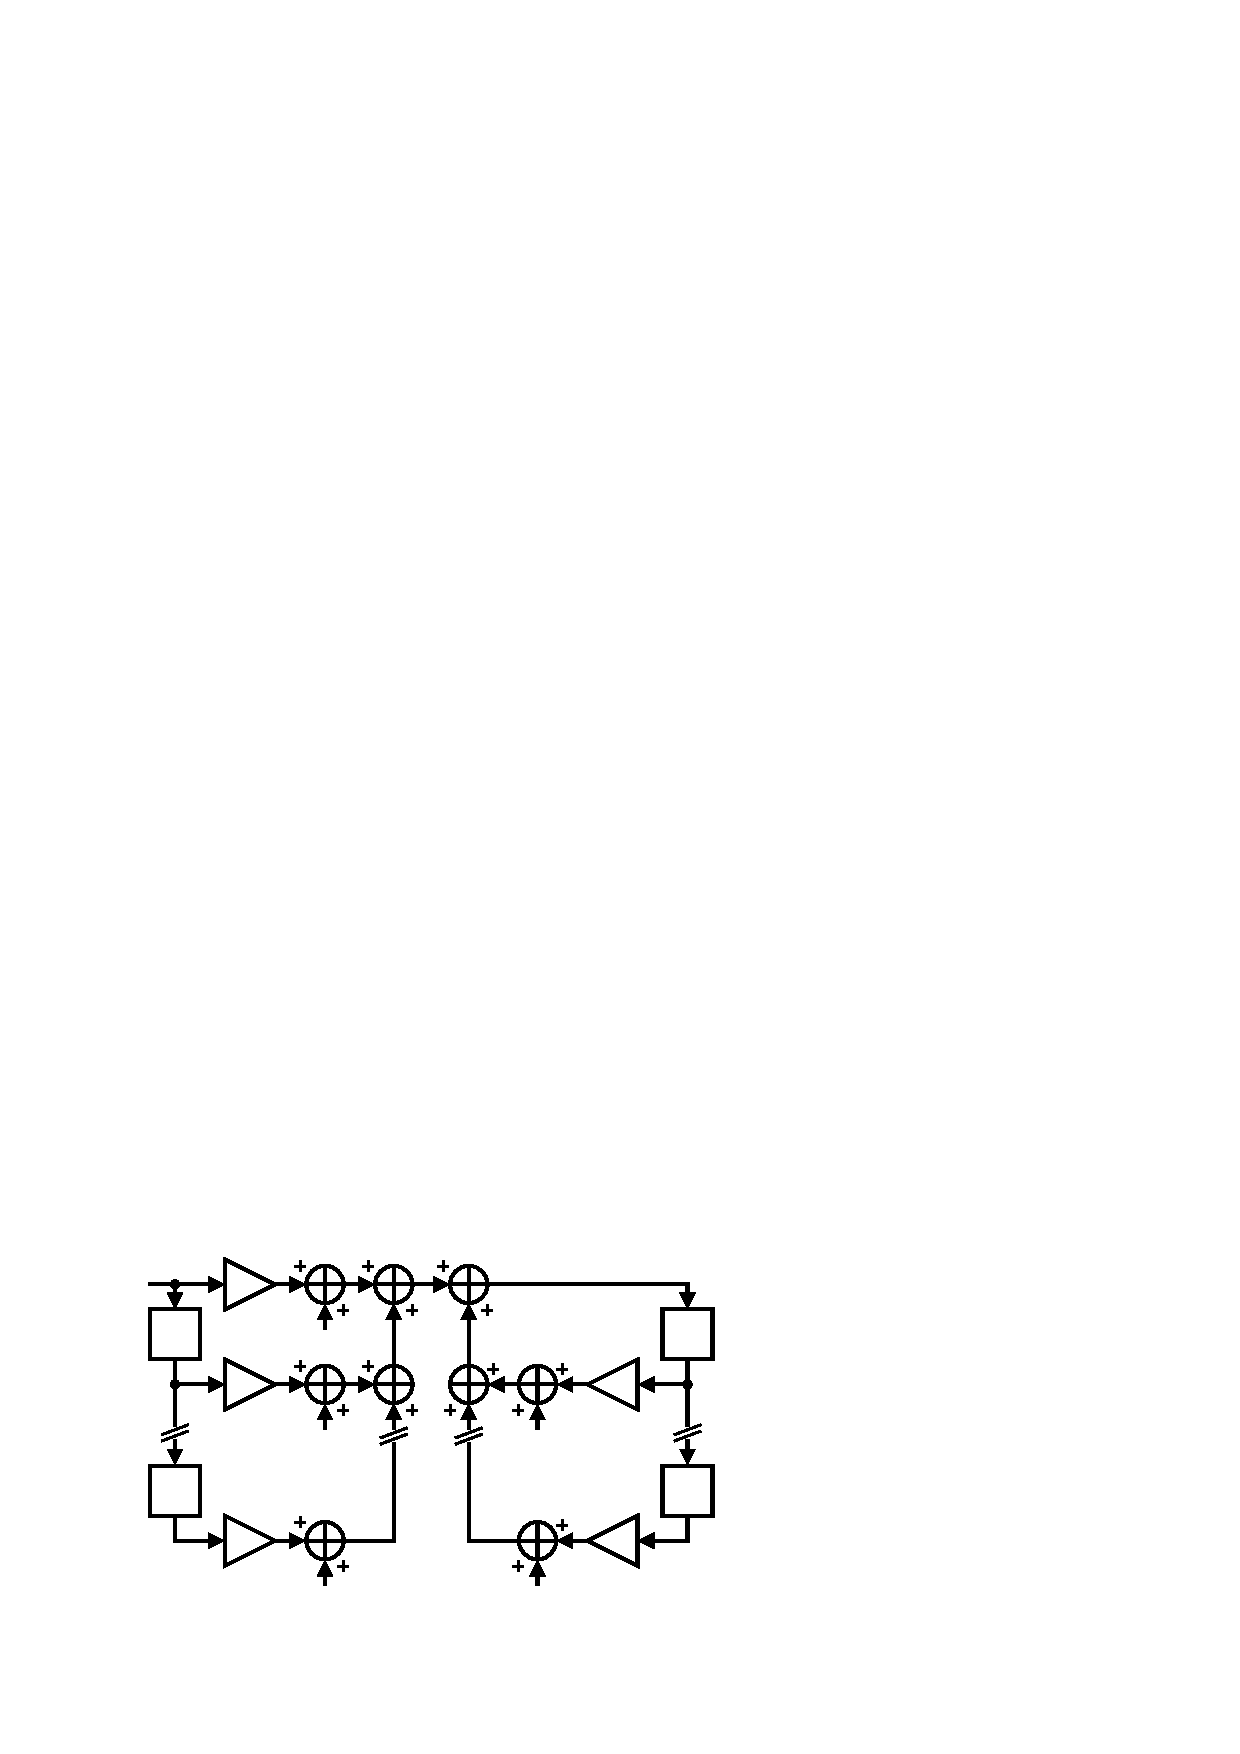
\includegraphics[scale=0.70000]{./figs/direct_type_1_quant.pdf}\\
   % translate x=936 y=1041 scale 0.38
   \putbox{0.05600in}{1.60300in}{0.96}{x[n]}%
   \putbox{2.60400in}{1.51900in}{0.96}{y[n]}%
   \putbox{0.05600in}{1.25300in}{0.96}{$z^{-1}$}%
   \putbox{0.51800in}{1.63100in}{0.96}{b$_0$}%
   \putbox{0.51800in}{1.16900in}{0.96}{b$_1$}%
   \putbox{2.44300in}{1.25300in}{0.96}{$z^{-1}$}%
   \putbox{2.44300in}{0.52500in}{0.96}{$z^{-1}$}%
   \putbox{2.03700in}{1.18300in}{0.96}{-a$_1$}%
   \putbox{2.02300in}{0.44800in}{0.96}{-a$_\mathrm{N}$}%
   \putbox{2.60400in}{1.05000in}{0.96}{y[n-1]}%
   \putbox{2.59000in}{0.32200in}{0.96}{y[n-2]}%
   \putbox{0.05600in}{0.52500in}{0.96}{$z^{-1}$}%
   \putbox{0.51800in}{0.43400in}{0.96}{b$_\mathrm{M}$}%
   \putbox{0.70700in}{1.25300in}{0.96}{q$_{b_0}$[n]}%
   \putbox{0.70700in}{0.78400in}{0.96}{q$_{b_1}$[n]}%
   \putbox{0.69300in}{0.05600in}{0.96}{q$_{b_\mathrm{M}}$[n]}%
   \putbox{1.68700in}{0.05600in}{0.96}{q$_{a_\mathrm{N}}$[n]}%
   \putbox{1.70100in}{0.78400in}{0.96}{q$_{a_1}$[n]}%
   } % close 'parbox'
   } % close 'scalebox'
   \vspace{-\baselineskip} % this is not necessary, but looks better
\fontfamily{\rmdefault}\selectfont

	        \caption{ }
	        \label{fig:direct_type_1_quant}
	    \end{subfigure}
	    % \caption{Approximate model for ring oscillator inverter delay cell.}
	    \label{fig:direct_type_1}
	    \caption{\textbf{(a)} Direct form I filter implementation, \textbf{(b)} With added quantization error signals.}
	\end{figure}
	Assuming the quantization error signals of each multiplier are uncorrelated with all other multipliers, the output-referred noise power of the filter can be computed as the sum of the output-referred individual contributions. These contributions can be determined via solving for the transfer function from each quantization noise source q$_x$[n] to the output y[n]. In the case of the direct form I filter structure, all quantization sources q$_x$[n] have the same transfer characteristic to the output y[n] given in equation \ref{eq:lf_quant_tf}.
	\begin{equation}
		\frac{Y(z)}{Q_x(z)} = \frac{1}{1+\sum_{k=1}^P a_kz^{-k}}\label{eq:lf_quant_tf}
	\end{equation}
	Applying the bilinear transform to equation \ref{eq:lf_quant_tf}, with high oversampling where P$\cdot \text{BW}_{loop} 10 < f_{ref}$, given P is the number of poles in the system:
	\begin{equation}
		\left.\frac{Y(z)}{Q_x(z)}\right\vert_{z^{-1}=1-sT} \approx \frac{1}{1+\sum_{k=1}^P a_k - s\sum_{k=1}^P ka_k}\label{eq:lf_quant_tf_s}
	\end{equation}
	The output power spectral density for each error source is, confined to a bandwidth defined by the (sampling) reference frequency $f_{ref}$:
	\begin{equation}
		S_{qx}(f) = \frac{\sigma_{qx}^2}{f_{ref}}\left|\frac{Y(s)}{Q_x(s)}\right|^2_{s=j2\pi f} \approx \frac{1}{12f_{ref}}\left|\frac{1}{1+\sum_{k=1}^P a_k - j2\pi f\sum_{k=1}^P ka_k}\right|^2 \hspace{1em}\frac{[\text{LSB}]^2}{[\text{Hz}]}
	\end{equation}
	Given P poles and Z zeros in the filter, the total output quantization PSD of the filter is in equation \ref{eq:lf_noise}. The total loop filter noise PSD linearly scales with the number of multipliers in the direct form I filter implementation.
	\begin{equation}
		S_{qn_{LF}}(f) = (P+Z+1)S_{qx}(f) \hspace{1em}\frac{[\text{LSB}]^2}{[\text{Hz}]}\label{eq:lf_noise}
	\end{equation}

\subsubsection{PLL Noise Sensitivity Transfer Functions}\label{ntfs}
	Having established models for noise of generated by each PLL component, noise sensitivity transfer functions must be computed to refer each noise source to the PLL output in terms of phase. In the noise theory presented here, all noise sources have been modeled as additive signal components. The full system model including all noise sources is in figure \ref{fig:full_pll_noise}.
	\begin{figure}[htb!]
		\center\fontfamily{\sfdefault}\selectfont
% XCircuit output "discrete_pll_full_noise.tex" for LaTeX input from discrete_pll_full_noise.ps
\def\putbox#1#2#3#4{\makebox[0.00000in][l]{\makebox[#1][l]{}\raisebox{\baselineskip}[0.00000in][0.00000in]{\raisebox{#2}[0.00000in][0.00000in]{\scalebox{#3}{#4}}}}}
\def\rightbox#1{\makebox[0.00000in][r]{#1}}
\def\centbox#1{\makebox[0.00000in]{#1}}
\def\topbox#1{\raisebox{-0.60\baselineskip}[0.00000in][0.00000in]{#1}}
\def\midbox#1{\raisebox{-0.20\baselineskip}[0.00000in][0.00000in]{#1}}
   \scalebox{1}{
   \normalsize
   \parbox{6.30000in}{
   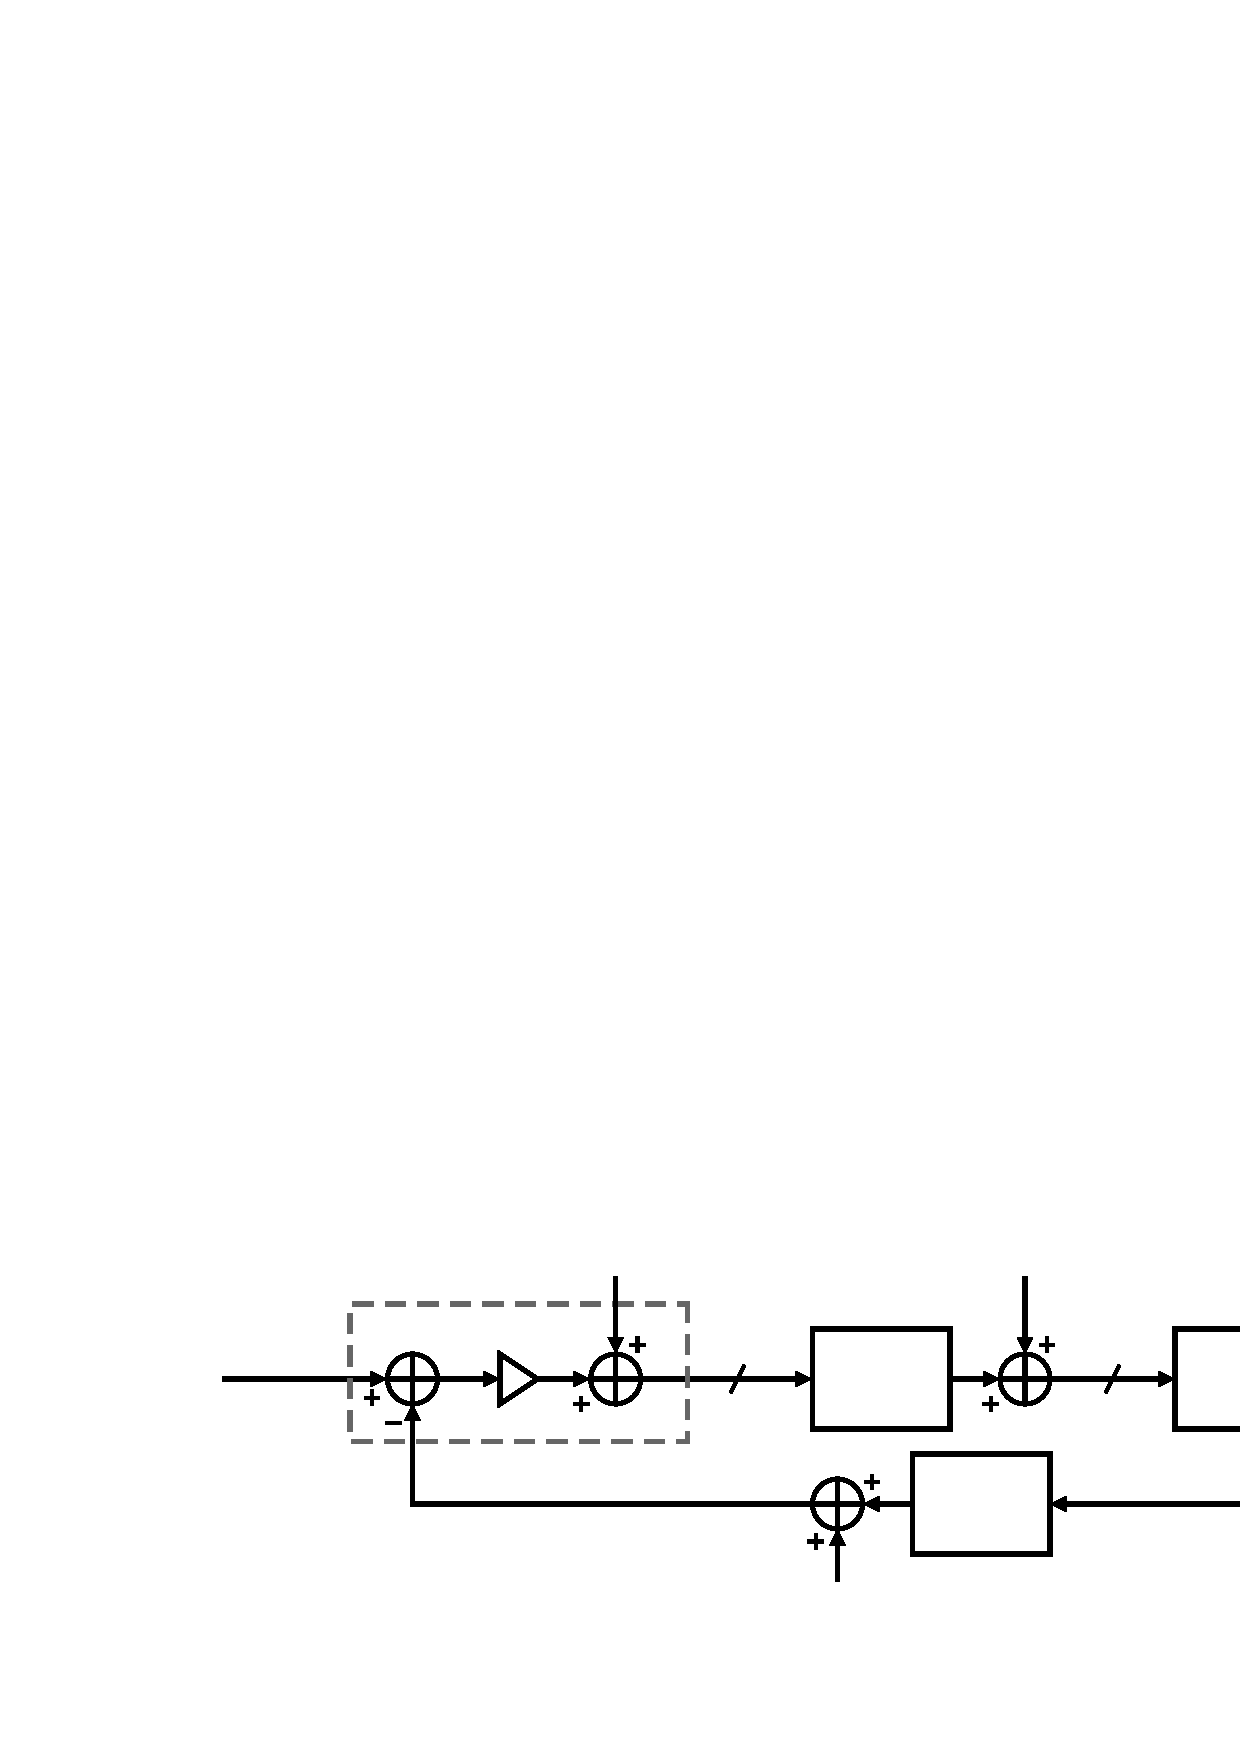
\includegraphics[scale=0.60000]{./figs/discrete_pll_full_noise.pdf}\\
   % translate x=416 y=544 scale 0.38
   \putbox{0.33600in}{1.00800in}{0.84}{$\Phi_{ref}$[n]}%
   \putbox{1.56000in}{0.51000in}{0.84}{$\Phi_{div}$[n]}%
   \putbox{2.27400in}{1.03200in}{0.84}{e$_\Phi$[n]}%
   \putbox{1.47000in}{1.07400in}{0.84}{\rotatebox{-360}{$\frac{\mathrm{M}}{2\pi}$}}%
   \putbox{1.20600in}{1.00800in}{0.84}{$\Phi_e$}%
   \putbox{0.83400in}{1.28400in}{0.84}{TDC}%
   \putbox{2.77200in}{0.89400in}{0.84}{H$_{LF}$(z)}%
   \putbox{3.79800in}{1.02000in}{0.84}{u[n]}%
   \putbox{4.22400in}{0.90600in}{0.84}{$\frac{2\pi K_{DCO}T}{1-z^{-1}}$}%
   \putbox{5.22000in}{0.99600in}{0.84}{$\Phi_{out}$[n]}%
   \putbox{3.22200in}{0.39600in}{0.84}{$\div$ N}%
   \putbox{4.13400in}{1.17000in}{0.84}{DCO}%
   \putbox{1.93200in}{1.30800in}{0.84}{q$_{n_{TDC}}$[n]}%
   \putbox{3.57000in}{1.30800in}{0.84}{q$_{n_{LF}}$[n]}%
   \putbox{2.82000in}{0.09600in}{0.84}{$\Phi_{n_{div}}$[n]}%
   \putbox{5.12400in}{1.30800in}{0.84}{$\Phi_{n_{DCO}}$[n]}%
   } % close 'parbox'
   } % close 'scalebox'
   \vspace{-\baselineskip} % this is not necessary, but looks better
\fontfamily{\rmdefault}\selectfont

		\caption{Full PLL additive noise model.}
		\label{fig:full_pll_noise}
	\end{figure}
	\FloatBarrier
	Following the approach of \cite{perrott_2002}, it is useful to define a transfer function $\hat{\mathrm{T}}(s)$ as in equation \ref{eq:parameterizing_tf} which characterizes the normalized closed loop response from reference input to output of the PLL. Normalized refers to the zero-frequency response being 1, i.e. $|\hat{\mathrm{T}}(0)|=1$. The noise transfer functions will be defined in this work in terms of $\hat{\mathrm{T}}(s)$. L(s) is the PLL loop gain. 
	\begin{equation}\label{eq:parameterizing_tf}
	\hat{\mathrm{T}}(s) = \frac{\mathrm{L}(s)}{1+\mathrm{L}(s)}\hspace{1em} \text{s.t.} \hspace{1em} \mathrm{T}(s) = \frac{\Phi_{out}}{\Phi_{ref}} = \mathrm{N}\hat{\mathrm{T}}(s) 
	\end{equation}
	Solving for the closed transfer functions between each noise source ($q_{n_{TDC}}$, $q_{n_{LF}}$, $\Phi_{n_{DCO}}$ and $\Phi_{n_{div}}$) to the output $\Phi_{out}$ in the s-domain yields equations \ref{eq:noise_tf_tdc}-\ref{eq:noise_tf_div}.
	\begin{align}
		\frac{\Phi_{out}(s)}{q_{n_{TDC}}(s)} & = \frac{2\pi\frac{K_{DCO}}{s}\mathrm{H}_{LF}(s)}{1+\mathrm{L}(s)}= 2\pi\frac{\mathrm{N}}{\mathrm{M}}\frac{\mathrm{L}(s)}{1+\mathrm{L}(s)} = 2\pi\frac{\mathrm{N}}{\mathrm{M}}\hat{\mathrm{T}}(s)\label{eq:noise_tf_tdc}\\
		\frac{\Phi_{out}(s)}{\Phi_{n_{DCO}}(s)} & = \frac{1}{1+\mathrm{L}(s)}= 1-\hat{\mathrm{T}}(s)\\
		\frac{\Phi_{out}(s)}{q_{n_{LF}}(s)} & = \frac{2\pi\frac{K_{DCO}}{s}}{1+\mathrm{L}(s)} = 2\pi\frac{K_{DCO}}{s}(1-\hat{\mathrm{T}}(s))\\
		\frac{\Phi_{out}(s)}{\Phi_{n_{div}}(s)} & = \frac{\mathrm{M}\frac{K_{DCO}}{s}\mathrm{H}_{LF}(s)}{1+\mathrm{L}(s)}= \mathrm{N}\frac{\mathrm{L}(s)}{1+\mathrm{L}(s)} = \mathrm{N}\hat{\mathrm{T}}(s)\label{eq:noise_tf_div}
	\end{align}


\subsubsection{PLL Phase Signal and Output PSD Relationship for Noise}\label{pn_noise_psd}
	When analyzing PLL noise in hardware, the noise power spectral density of the PLL output waveform is the most relevant metric. Up to this point, noise has been defined in terms of phase signal $\Phi_{n}$, or an unwanted added component to the oscillator phase signal $\Phi_{osc}=\omega_{osc}t$. The PLL output phase signal $\Phi_{out}$ is thus:
	\begin{equation}
		\Phi_{out}(t) = \Phi_{osc}(t) + \Phi_{n}(t) = \omega_{osc}t + \Phi_{n}(t) 
	\end{equation}
	To determine the PSD of the PLL output waveform, a definition of the PLL output voltage waveform will be made in terms of a sinusoid, i.e. the real portion of a complex exponential. Given an oscillation amplitude $A_0$:
	\begin{equation}
		V_{out} = \Re\left(A_0e^{j\Phi_{out}(t)}\right) = \Re\left(A_0e^{j\omega_{osc}t}e^{j\Phi_{n}(t)}\right)
	\end{equation}
	Assuming the phase noise signal is zero mean, $\mathbb{E}[\Phi_{n}(t)]=0$, and the power of phase noise signal is small, $\mathrm{Var}[\Phi_{n}(t)] << 1$, then the approximation $e^{j\Phi_{n}(t)} = 1 + j\Phi_{n}(t)$ can be applied by truncating the exponential Taylor series expansion.
	\begin{align}
		V_{out} &= \Re\left(A_0e^{j\omega_{osc}t}e^{j\Phi_{n}(t)}\right) = \Re\left(A_0e^{j\omega_{osc}t} +j\Phi_{n}(t)A_0e^{j\omega_{osc}t}\right)\\
		&= A_0\cos(\omega_{osc}t) - \Phi_{n}(t)A_0\sin(\omega_{osc}t) \label{eq:pll_out_approx}
	\end{align}
	The result is a carrier cosine signal, and an orthogonal sine signal modulated by the phase noise $\Phi_{n}$. From this, the spectral density of the phase noise relative to the carrier can be estimated. The power spectral density $S_{V_{out}}$ is computed in equations \ref{eq:psd_vout}-\ref{eq:psd_noise}. Due to orthogonality of the sine/cosine components of equation \ref{eq:pll_out_approx}, the cross terms that appear in the PSD computation are zero. 
	\begin{align}
		S_{V_{out}}(f) =& \lim_{\Delta T\rightarrow\infty}\frac{1}{\Delta T}|\mathcal{F}\{V_{out}(t)\cdot\mathrm{rect}(t/\Delta T)\}|^2 \label{eq:psd_vout}\\
		=&\lim_{\Delta T\rightarrow\infty}\frac{A_0^2}{\Delta T}|\mathcal{F}\{\cos(\omega_{osc}t)\cdot\mathrm{rect}(t/\Delta T)\}|^2 \label{eq:psd_carrier}\\ 
		&+ \lim_{\Delta T\rightarrow\infty}\frac{A_0^2}{\Delta T}|\mathcal{F}\{\Phi_{n}(t)\cdot\mathrm{rect}(t/\Delta T)\}*\mathcal{F}\{\sin(\omega_{osc}t)\cdot\mathrm{rect}(t/\Delta T)\}|^2 \label{eq:psd_noise}
	\end{align}
	 The noise power spectral density function of the output waveform $\mathcal{L}(\Delta f)$ is defined as the noise PSD at offset $\Delta f$ from the carrier frequency $f_{osc}$, normalized to the carrier power. Here the PSD of the carrier component is given by equation \ref{eq:psd_carrier}, and the noise component by equation \ref{eq:psd_noise}. Shifting equation \ref{eq:psd_noise} by $-\omega_{osc}$ and performing normalization for carrier power results in:
	\begin{equation}\label{eq:pn_psd_relation}
		\mathcal{L}(\Delta f) = \left.\lim_{\Delta T\rightarrow\infty}\frac{1}{\Delta T}|\mathcal{F}\{\Phi_{n}(t)\cdot\mathrm{rect}(t/\Delta T)\}|^2 \right|_{f=\Delta f}= S_{\Phi_{n}}(\Delta f)
	\end{equation}

	Thus, the noise PSD $\mathcal{L}(\Delta f)$ of the PLL output waveform relative to the carrier is equal to the PSD of the phase noise signal $\Phi_{n}(t)$, provided $\text{Var}[\Phi_{n}(t)] << 1$. The PSD of $\Phi_{n}(t)$ is notated as $S_{\Phi_{n}}(\Delta f)$.

\subsubsection{PLL Output-Referred Noise PSD}\label{final_pn_model}
To compute the PLL output noise PSD, the individual PLL noise sources must be referred to the PLL output. Thus far the following have been established: (a) noise spectrum generated by each individual PLL component, (b) the PLL phase noise sensitivity functions, and (c) the relationship between output phase noise and the PSD of the PLL output waveform. These can be combined to provide a final result for total PLL output-referred noise PSD. An assumption here is all noise sources are uncorrelated, so their independent noise power contributions may be summed to find the total noise PSD. The PLL output phase noise PSD for each noise source is simply found by multiplying the magnitude squared of the respective noise sensitivity function with the noise source PSD. Thus:
\begin{align}
	S_{\Phi n_{TDC,out}}(f) &= S_{qn_{TDC}}(f)\left|\frac{\Phi_{out}(f)}{q_{n_{TDC}}(f)}\right|^2 = \frac{1}{12f_{ref}}\left|2\pi\frac{\mathrm{N}}{\mathrm{M}}\hat{\mathrm{T}}(f)\right|^2\label{eq:tdc_pn_psd}\\
	S_{\Phi n_{DCO,out}}(f) &= S_{\Phi n_{DCO}}(f)\left|\frac{\Phi_{out}(f)}{\Phi_{n_{DCO}}(f)}\right|^2  = \frac{S_{0\Phi n_{DCO}}}{f^2}\left|1-\hat{\mathrm{T}}(f)\right|^2\\		
	S_{\Phi n_{LF,out}}(f) &= S_{q n_{LF}}(f)\left|\frac{\Phi_{out}(f)}{q_{n_{LF}}(f)}\right|^2 \approx \frac{K_{DCO}^2}{12f_{ref}f^2}\frac{(P+Z+1)|1-\hat{\mathrm{T}}(f)|^2}{\left|1+\sum_{k=1}^P a_k - j2\pi f\sum_{k=1}^P ka_k\right|^2}\\
	S_{\Phi n_{div,out}}(f) &= S_{\Phi n_{div}}(f)\left|\frac{\Phi_{out}(f)}{\Phi_{n_{div}}(f)}\right|^2 = f_{ref}\left|2\pi\sigma_{tn_{div}}\mathrm{N}\hat{\mathrm{T}}(f)\right|^2\label{eq:div_pn_psd}\
\end{align}
The final PLL output noise PSD at offset $\Delta f$ relative to the carrier frequency and normalized to carrier power of PLL will be:
\begin{equation}
	\mathcal{L}(\Delta f) = S_{\Phi n_{TDC,out}}(\Delta f) + S_{\Phi n_{DCO,out}}(\Delta f) + S_{\Phi n_{LF,out}}(\Delta f) + S_{\Phi n_{div,out}}(\Delta f)
\end{equation}

\subsection{Bang-bang phase detector PLL}\label{bbpd_theory}
% First reference : \cite{toifl_1998}
\vspace{-1em}
\begin{figure}[htb!]
	\center\include{./figs/bbpll}
	\caption{PLL with bang-bang phase detector.}
	\label{fig:bbpll}
\end{figure}
An alternative digital phase detector that is not resolution limited like a TDC is the bang-bang phase detector (BBPD) \cite{zanuso_2009}. A BBPD is implemented in a PLL as shown in figure \ref{fig:bbpll}. The BBPD in principle functions by outputting a 1 if the divider signal is late relative to the clock, and -1 if it is early. A BBPD exhibits hard nonlinearity in its transfer characteristics. However, as shown in \cite{xu_abidi_2017}, a linearized model for BBPD gain can be established, given in equation \ref{eq:nom_bbpd_gain} if the signal variance $\sigma_{\Phi_e}^2$ into the detector is constant. Here the input to the detector is phase error signal $\Phi_e=\Phi_{CLK}-\Phi_{DIV}$ and the output $\mathrm{y}$ valued as $\pm 1$ (its variance $\sigma_y^2$=1).
\begin{equation}\label{eq:nom_bbpd_gain}
	K = \frac{\mathbb{E}[\Phi_e(t)\cdot\mathrm{y}(t)]}{\mathbb{E}[\Phi_e^2(t)]} = \sqrt{\frac{2}{\pi}}\frac{1}{\sigma_{\Phi_e}}
\end{equation}
The noise power of the BBPD can be determined as $\sigma_{n_{BBPD}}^2$ = $\sigma_y^2$ - $K^2\sigma_{\Phi_e}^2$ = $1-\frac{2}{\pi}$. It is observed that the BBPD noise power is fixed, unlike the TDC, which can reduce the limitations on detector phase noise compared to the quantization prone TDC. Given the BBPD samples the divider phase at a rate equal to $f_{ref}$, the BBPD noise spectral density is in equation \ref{eq:bbpd_noise_psd}. The gain of the BBPD, however, changes with input signal variance, which affects the PLL loop gain and thus closed loop PLL response. The variance of the signal into the phase detector should be expected to vary across PLL process, voltage and temperature conditions, thus the BBPD is limited in terms of gain accuracy. The linearized gain and noise values determined here can be substituted for the TDC model established for PLL transfer function and phase noise in sections \ref{adpll_model} and \ref{pn_theory} to solve for BBPD-PLL dynamics. This yields the closed loop response of equation \ref{eq:cl_bbpd_pll}, the noise transfer function in equation \ref{eq:ntf_bbpd_pll}, and the output-referred noise spectral density in equation \ref{eq:out_psd_bbpd_pll}.
\begin{equation}\label{eq:bbpd_noise_psd}
	S_{ n_{BBPD}(f)} = \frac{\sigma_{n_{BBPD}}^2}{\Delta f} = \frac{\left(1-\frac{2}{\pi}\right)}{f_{ref}}
\end{equation}
	\begin{align}\label{eq:cl_bbpd_pll}
		\mathrm{T}(s)=\frac{\Phi_{out}(s)}{\Phi_{ref}(s)} = \frac{2\pi \sqrt{\frac{2}{\pi}}\frac{1}{\sigma_{\Phi_e}}K_{DCO}\sum_{j=0}^Z b_js^j}{\sum_{k=0}^P a_ks^{k+1} + 2\pi \sqrt{\frac{2}{\pi}}\frac{\mathrm{1}}{\sigma_{\Phi_e}\mathrm{N}}K_{DCO}\sum_{j=0}^Z b_js^j} = \mathrm{N}\frac{\mathrm{L}(s)}{1+\mathrm{L}(s)}
	\end{align}
\begin{align}\label{eq:ntf_bbpd_pll}
	\frac{\Phi_{out}(f)}{n_{{BBPD}}(f)} = \sqrt{\frac{\pi}{2}}\sigma_{\Phi_e}\mathrm{N}\frac{\mathrm{L}(f)}{1+\mathrm{L}(f)} = \sqrt{\frac{\pi}{2}}\sigma_{\Phi_e}\mathrm{N}\hat{\mathrm{T}}(f)
\end{align}
\begin{align}\label{eq:out_psd_bbpd_pll}
	S_{\Phi n_{BBPD,out}}(f) &= S_{n_{BBPD}}(f)\left|\frac{\Phi_{out}(f)}{q_{n_{BBPD}}(f)}\right|^2 = \frac{\left(\frac{\pi}{2}-1\right)}{f_{ref}}\left|\sigma_{\Phi_e}\mathrm{N}\hat{\mathrm{T}}(f)\right|^2
\end{align}
% Out PSD = Noise PSD * |(TF from source to output)|^2

% out PSD = sum of individual PSDs



	% \section{Methods}\label{methods}
	\pagebreak
	\section{Methods}\label{methods}
The methods for simulation of the discrete-time 

\hl{Talk about how simulator is implemented:}
\hl{Discrete simulation models of phase noise, dco etc}
\hl{Filter optimization}
\hl{-phase noise and lock time estimate in frequency domain}

\hl{Design recommendations:}
\hl{High sampling rate}
\hl{Minimum choice of TDC tesolution, constraints for divider jitter,}
\subsection{Behavioral, discrete event PLL simulation}
\subsubsection{Phase noise modeling}
\subsubsection{Measurement of phase noise, spurs}
\subsubsection{Monte-carlo sampling}
	\hl{Used to verify stability}

\subsection{Loop filter optimization}
	Reference phase noise does not matter, is always fixed.
	DCO and TDC phase noise should be highest. Will simulate with other noise sources, but framework will optimize loop filter design and provide recommendations for other parameters (max divider jitter) so DCO and TDC phase noise are dominant.
\subsubsection{Estimation of settling time}

	Based on a continuous model of the PLL dynamics, the PLL closed loop phase transfer function $\mathrm{T}(s)$ is defined in the following form, where number of poles P $>$ number of zeros Z. The transfer function is defined as a rational function of two polynomial functions of s. 
	\begin{equation}\label{eq:pll_cl_tf}
	\mathrm{T}(s) = \frac{\sum_{j=0}^Z b_js^j}{\sum_{k=0}^P a_ns^n}
	\end{equation}
	An estimate of the step response settling time of $\mathrm{T}(s)$ can by utilizing its representation in state space. This is given in \ref{eq:ss_rep}, with input vector $\mathrm{U}(s)$, state vector $\mathbf{X}(s)$,  and output $\mathbf{Y}(s)$. The state-space representation from a s-domain transfer function can be quickly solved computationally with available signal processing packages such as \texttt{scipy.signal}.
	% https://lpsa.swarthmore.edu/Representations/SysRepTransformations/TF2SS.html
	\begin{align} \label{eq:ss_rep}
		s\mathbf{X}(s) &= \mathbf{AX}(s) +\mathbf{B}\mathrm{U}(s)\\
		Y(s) &= \mathbf{CX}(s) +\mathbf{D}\mathrm{U}(s)
	\end{align}
	The set of k eigenvalues $\{\lambda_1, ... , \lambda_{N}\}$ corresponding to poles for the system are found as the roots of \ref{eq:ss_eigenvals}.% The associated eigenvectors are found with \ref{eq:ss_eigenvecs}.
	\begin{align}
		|\mathbf{A} - \lambda \mathbf{I}| = 0\label{eq:ss_eigenvals}%\\
		%\mathbf{A} \mathbf{v}_k = \lambda_k\mathbf{v}_k \label{eq:ss_eigenvecs}
	\end{align}
	With the constraint of number of poles $>$ number of zeros, the system $\mathrm{T}(s)$ may be represented via partial fraction decomposition using the poles from the eigenvalues of state matrix $\mathbf{A}$ $\{\lambda_1, ... , \lambda_{N}\}$:
	\begin{equation}
		T(s) = \sum_{k=1}^{P} \frac{c_k}{s-\lambda_k}
	\end{equation}
	The step response of this system will take the form as a sum of complex exponentials:
	\begin{equation}
		y(t) = c_1e^{\lambda_1t} + ... + c_ke^{\lambda_kt}%, \hspace{1em} \mathbf{y(t)} = [ y(t) \hspace{0.5em}y^{'}(t)\hspace{0.5em} ...\hspace{0.5em} y^{(k)}(t)]^T
	\end{equation}

	% The state transition matrix $\mathbf{\Phi}_{\mathrm{T}}$ corresponding to the system $\mathrm{T}(s)$ is:
	% \begin{equation}
		% \mathbf{\Phi}_\mathrm{T} = (s\mathbf{I}-A)^{-1}
	% \end{equation}

	The dynamics of the step response are governed by the exponential components of y(t). If  $\{\lambda_1, ... , \lambda_N\} \in \mathds{C}$ where $\lambda_k=\sigma_k+j\omega_K$, the real portion of each $\lambda_k$ will describe the transient behavior. The long term settling of y(t) will be dominated by the $\lambda_k$ with the smallest valued real component, that is the dominant pole. This value is approximately the reciprocal time constant for the system. Settling time $t_s$ can be considered as the interval required for the signal to drop within a tolerance band $\pm \delta_{tol} \textnormal{y}(\infty)$ about the final value $\textnormal{y}(\infty)$. 
	\begin{equation}
		t_s = \tau\ln(\delta_{tol}) = \frac{\ln(\delta_{tol})}{\min(|\Re(\{\lambda_1, ... , \lambda_k\})|)}
	\end{equation}
	This settling time estimate is computationally fast, as it requires only (a) computation of state matrix $\mathbf{A}$, (b) computation of the eigenvalues of $\mathbf{A}$, and (c) computation of settling time from the eigenvalue with minimum real component.
\subsubsection{Estimation of PLL phase noise}
	It is assumed that the dominant output-referred phase noise contributions are due to the DCO thermal noise and the TDC quantization. If such is the case, total output integrated noise power is at a minimimum when the TDC and DCO contributions are approximately equal. Thus $S_{TDC}$ and $S_{DCO}$ are the PLL output-referred noise PSD respectively for the TDC and DCO noise sources. The total PLL output noise PSD $S_{\Sigma}(f)$ is (N is the PLL divider modulus):
	\begin{equation}
		S_{\Sigma}(f) = f_{clk}\cdot|2\pi N\cdot G(f)|^2S_{TDC} + |1-G(f)|^2S_{DCO}
	\end{equation}

	Given a bandwidth of interest $\Delta f$ (i.e. baseband bandwidth for radio applications), the total integrated phase noise power is:
	\begin{equation}
		P_{\phi noise} = 2\int_0^{\Delta f} S_{\Sigma}(f)df
	\end{equation}
	This can be computation solved for a grid of K values in the interval $\Delta f$, where each point represents a frequency bin $f_{bin}$ = $\Delta f$/K. Therefore this estimate is implemented as such:
	\begin{equation}
		\hat{P}_{\phi noise} = 2\sum_{k=0}^{K-1} S_{\Sigma}(kf_{bin})f_{bin}
	\end{equation}

\subsubsection{Optimization algorithm}
	Utilize BFGS optimization with constraints on settling time


    % \section{Results}
    \pagebreak
	\section{Discussion and results}\label{disco}
    Thus far in this work a solution to simplify and automate design the process of all digital PLL loop filter designs comprised of (1) an automated loop filter optimization and design engine, and (2) a discrete-event, time domain PLL simulator to evaluate the designed filters with full time-discretization and quantization nonlinearity effects. Now, in this discussion, the performance of the presented design solution will first be evaluated with a design example. Then, a comparison of the presented solution then will be made to existing solutions in literature, pointing out advantages and disadvantages will be made. Finally, a general discussion will be made covering areas of improvement, reasoning for the central design choices made, and considerations for usage the framework.

\subsection{Design exercise using this work}
The design of a loop filter for the PLL with the system level specifications of table \ref{design_specs} will be considered here, with the intent of optimizing phase noise. These specifications, where the TDC resolution in steps equals the divider ratio, is equivalent to a special case of a TDC-less PLL where a 150-step synchronous counter is used as a divider, and the loop filter directly samples the state of the synchronous counter. For filter design, a PI-controller loop filter prototype was utilized in the optimizer.

% \scriptsize
\begin{table}[h!]
	\centering
	\def\arraystretch{1.5}		
	\setlength\arrayrulewidth{0.75pt}
	\setlength{\tabcolsep}{1em} % for the horizontal padding
	\begin{tabular}{|l|r|l|}
		\hline 
		\rule[-1ex]{0pt}{2.5ex} \cellcolor{gray!40}\textbf{Parameter} & \cellcolor{gray!40}\textbf{Value} & \cellcolor{gray!40}\textbf{Unit }\\ 
		\hline 
		\rule[-1ex]{0pt}{2.5ex} \textbf{Output Frequency}  & 2.4 & GHz \\ 
		\hline 
		\rule[-1ex]{0pt}{2.5ex} \textbf{Ref. frequency} & 16 & MHz\\ 
		\hline 
		\rule[-1ex]{0pt}{2.5ex} \textbf{Divider ratio} & 150  &\\ 
		\hline 
		\rule[-1ex]{0pt}{2.5ex} \textbf{TDC resolution} & 150  & steps/reference cycle\\ 
		\hline 
		\rule[-1ex]{0pt}{2.5ex} \textbf{DCO gain $K_{DCO}$} & $10^4$ & Hz/LSB \\ 
		\hline 
		\rule[-1ex]{0pt}{2.5ex} \textbf{DCO Phase noise} & -80 & dBc/Hz at $\Delta f=10^6$ Hz \\ 
		\hline 
		\rule[-1ex]{0pt}{2.5ex} \textbf{Lock Time} & $\leq$ 25 & $\mu$s \\ 
		\hline 
		\rule[-1ex]{0pt}{2.5ex} \textbf{Lock $\Delta f$ tolerance} & $10^5$ & Hz \\ 
		\hline 
		\rule[-1ex]{0pt}{2.5ex} \textbf{Digital filter word resolution} & $\leq$ 16 & bits \\ 
		\hline 
		\rule[-1ex]{0pt}{2.5ex} \textbf{Residual phase modulation} & minimize &  \\ 
		\hline 
	\end{tabular} 
	% \caption{Assigned specifications for branch line hybrid design.}
	% \label{asgn_specs}
	\caption{System-level specifications}
	\label{design_specs}
\end{table}   

\subsubsection{Result of filter optimization.}
Table \ref{filter_params} contains the optimized filter parameters obtained from the filter design optimizer developed in this work. $\{K$, $K_i$, $K_p$, $f_z\}$ are the continuous model parameters of section \ref{cont_pi_filt_des}, and $\{a_0$, $a_1$, $a_2$, $b_0$, $b_1\}$ are the filter coefficients for the discrete-time direct form-I filter structure of section \ref{disc_lf_comp_pi}. The estimated bandwidth for the filter is 144.8 kHz, and the lock time is estimated to be 19.3 $\mu$s. Table \ref{dig_filter_params} contains the digitized version of the discrete time filter, based on a selection for word size determined via optimization for finite word effects. The final data words are 13 bits in length.  
% \scriptsize
\begin{table}[h!]
	\centering
	\def\arraystretch{1.5}		
	\setlength\arrayrulewidth{0.75pt}
	\setlength{\tabcolsep}{1em} % for the horizontal padding
	\begin{tabular}{|l|r|l|}
		\hline 
		\rule[-1ex]{0pt}{2.5ex} \cellcolor{gray!40}\textbf{Parameter} & \cellcolor{gray!40}\textbf{Value} & \cellcolor{gray!40}\textbf{Unit }\\ 
		\hline 
		\rule[-1ex]{0pt}{2.5ex} \textbf{$K$}  & $1.343792\times10^{11}$ &  \\ 
		\hline 
		\rule[-1ex]{0pt}{2.5ex} \textbf{$K_i$}  & $1.343792\times10^{7}$ &  \\ 
		\hline 
		\rule[-1ex]{0pt}{2.5ex} \textbf{$K_p$}  & $7.331074\times10^{1}$ &  \\ 
		\hline 
		\rule[-1ex]{0pt}{2.5ex} \textbf{$f_z$} & $2.917324\times10^4$ & Hz\\ 
		\hline 
		\rule[-1ex]{0pt}{2.5ex} \textbf{$b_0$}  & $7.4150613906\times10^1$  &\\ 
		\hline 
		\rule[-1ex]{0pt}{2.5ex} \textbf{$b_1$}  & $-7.3310743796\times10^1$  & \\ 
		\hline 
		\rule[-1ex]{0pt}{2.5ex} \textbf{$a_0$}  & $1.0\times10^0$  &\\ 
		\hline 
		\rule[-1ex]{0pt}{2.5ex} \textbf{$a_1$}  & $-1.0\times10^0$  & \\ 
		\hline 
		\rule[-1ex]{0pt}{2.5ex} \textbf{$a_2$}  & $0.0\times10^0$  & \\ 
		\hline 
		\rule[-1ex]{0pt}{2.5ex} Estimated bandwidth & $1.448234\times10^5$ & Hz \\ 
		\hline 
		\rule[-1ex]{0pt}{2.5ex} Estimated lock time & $1.934253\times10^{-5}$ & seconds \\ 
		\hline 
	\end{tabular} 
	% \caption{Assigned specifications for branch line hybrid design.}
	% \label{asgn_specs}
	\caption{PLL parameters determined from filter design and optimization process.}
	\label{filter_params}
\end{table}   

\begin{table}[h!]
	\centering
	\def\arraystretch{1.5}		
	\setlength\arrayrulewidth{0.75pt}
	\setlength{\tabcolsep}{1em} % for the horizontal padding
	\begin{tabular}{|l|r|r|l|}
		\hline 
		\rule[-1ex]{0pt}{2.5ex} \cellcolor{gray!40}\textbf{Parameter} & \cellcolor{gray!40}\textbf{Value} & \cellcolor{gray!40}\textbf{Value (digital) } & \cellcolor{gray!40}\textbf{Value Error}\\ 
		\hline 
		\rule[-1ex]{0pt}{2.5ex} Total dataword bits  & 13 & & \\ 
		\hline 
		\rule[-1ex]{0pt}{2.5ex} Sign bits  & 1 & & \\ 
		\hline 
		\rule[-1ex]{0pt}{2.5ex} Integer bits & 7 & & \\ 
		\hline 
		\rule[-1ex]{0pt}{2.5ex} Fractional bits  & 5 & & \\ 
		\hline 
		\rule[-1ex]{0pt}{2.5ex} \textbf{$b_0$} & $7.415625\times10^1$ & \texttt{0b0100101000101}  & $+5.636094\times10^{-3}$\\ 
		\hline 
		\rule[-1ex]{0pt}{2.5ex} \textbf{$b_1$}  & $-7.331250\times10^1$ & \texttt{0b1111011010110}  & $-1.756204\times10^{-3}$\\ 
		\hline 
		\rule[-1ex]{0pt}{2.5ex} \textbf{$a_0$}  & $1.0\times10^0$ & \texttt{0b0000000100000} & $0.0\times10^0$ \\ 
		\hline 
		\rule[-1ex]{0pt}{2.5ex} \textbf{$a_1$}  & $-1.0\times10^0$ & \texttt{0b1111111100000} & $0.0\times10^0$ \\ 
		\hline 
		\rule[-1ex]{0pt}{2.5ex} \textbf{$a_2$}  & $0.0\times10^0$ & \texttt{0b0000000000000} & $0.0\times10^0$ \\ 
		\hline 
	\end{tabular} 
	% \caption{Assigned specifications for branch line hybrid design.}
	% \label{asgn_specs}
	\caption{Loop filter parameters after digitization and optimization for data word length.}
	\label{dig_filter_params}
\end{table}  

\subsubsection{Result of transient and phase noise simulation.}
The simulation engine implemented in this work was utilized to run a time domain simulation to verify the designed filter. Figures \ref{fig:trans_lf} and \ref{fig:trans_inst_freq} demonstrate the transient response of the PLL with an initial frequency error of 12 MHz (0.5\% of final frequency). It is observed that the PLL design stably approaches the target frequency in approximately 23 $\mu$s. Figures \ref{fig:trans_det} illustrate the BBPD and TDC outputs during this inital transient. It is observed that the TDC output gives the dominant feedback, unit it reaches an output word of 0, where the BBPD then begins providing feedback in the steady state condition of the PLL. Figure \ref{fig:trans_phase_noise} is the result of a phase noise calculation for the simulated PLL in an interval beginning immediately after detection of lock. The spectrum closely approximates that designed for, with some small additional peaking.
	\begin{figure}[htb!]
	    \centering
	    \begin{subfigure}{0.5\textwidth}
	        \centering
	        \center\includegraphics[width=1.0\textwidth, angle=0]{figs/trans_loop_filter.pdf}
	        \caption{ }
	        \label{fig:trans_lf}
	    \end{subfigure}%
	    \begin{subfigure}{0.5\textwidth}
	        \centering
	        \center\includegraphics[width=1.0\textwidth, angle=0]{figs/trans_inst_freq.pdf}
	        \caption{ }
	        \label{fig:trans_inst_freq}
	    \end{subfigure}
	    % \caption{Approximate model for ring oscillator inverter delay cell.}
	    \label{fig:trans_sim1}
	    \caption{Simulation with 0.5\% initial frequency error: \textbf{(a)} Loop filter transient response, \textbf{(b)} PLL output instantaneous frequency.}
	\end{figure}

	\begin{figure}[htb!]
	    \centering
	    \begin{subfigure}{0.5\textwidth}
	        \centering
	        \center\includegraphics[width=1.0\textwidth, angle=0]{figs/trans_tdc_bbpd.pdf}
	        \caption{ }
	        \label{fig:trans_det}
	    \end{subfigure}%
	    \begin{subfigure}{0.5\textwidth}
	        \centering
	        \center\includegraphics[width=1.0\textwidth, angle=0]{figs/trans_phase_noise.pdf}
	        \caption{ }
	        \label{fig:trans_phase_noise}
	    \end{subfigure}
	    % \caption{Approximate model for ring oscillator inverter delay cell.}
	    \label{fig:trans_sim2}
	    \caption{Simulation with 12 MHz (0.5\%) initial frequency error: \textbf{(a)} BBPD/TDC detector responses, \textbf{(b)} PLL output phase noise power spectrum.}
	\end{figure}

\subsubsection{Result of parametric sweep and variation analysis.}
The Monte-Carlo sampling and parametric sweep facilities in the simulator designed in this work were used to run analysis for effects of variation of DCO gain $K_{DCO}$ and initial frequency error of the PLL. Figure \ref{fig:sweep_kdco} shows a parametric sweep of $K_{DCO}$, with lock time being measured. It is observed that the lock time is nearly flat in the range 7300-18000 Hz/LSB, meaning that there is a tolerance of -2700/+8000 Hz LSB for KDCO about the nominal 10000 Hz/LSB specified. This specification can be utilized in the design of a physical DCO to constrain maximum acceptable variation across PVT. Figure \ref{fig:sweep_finit} demonstrates the simulated effect of initial frequency error on lock time. It is seen that PLL stably locks to the target frequency within the entire simulated interval of $\pm$ 60 MHz from 2.4GHz, implying that the capture range of the PLL is $>120$ MHz. This specification can be translated into a requirement for initial coarse frequency calibration needed before starting the PLL. Figures \ref{fig:mc_trans} and \ref{fig:mc_hist} are the results of a variation analysis simulation utilizing the Monte-Carlo sampling engine implemented in this work. The simulation was configured to vary $K_{DCO}$ with a standard deviation of 20 \% of the nominal value, and to vary the inital starting frequency with a standard deviation of 60 MHz (0.025 \% of the final frequency). The simulation sample size is 1000. The transient responses from the simulation figure \ref{fig:mc_trans} are all stable, and figure \ref{fig:mc_hist} shows the histogram for measured lock time subject to the described variation. The mean lock time was 24.57 $\mu$s, meeting the 25 $\mu$s lock time set for the PLL, and the upper bound for a 99\% confidence interval on the data is 50.75 $\mu$s. A set of extracted parameters from these simulations are in table \ref{simulation_params}. The Monte-Carlo simulations presented here are useful to analyze the range of variation in which the designed PLL can tolerate, as well as determine the expected performance varation, so well informed decisions on a PLL design can be made before moving into transistor level implementation and simulation. 

	\begin{figure}[htb!]
	    \centering
	    \begin{subfigure}{0.5\textwidth}
	        \centering
	        \center\includegraphics[width=1.0\textwidth, angle=0]{figs/_kdco_sweep.pdf}
	        \caption{ }
	        \label{fig:sweep_kdco}
	    \end{subfigure}%
	    \begin{subfigure}{0.5\textwidth}
	        \centering
	        \center\includegraphics[width=1.0\textwidth, angle=0]{figs/_finit_sweep.pdf}
	        \caption{ }
	        \label{fig:sweep_finit}
	    \end{subfigure}
	    % \caption{Approximate model for ring oscillator inverter delay cell.}
	    \label{fig:sweep_sim}
	    \caption{\textbf{(a)} PLL lock time simulation with KDCO swept, 12 MHz (0.5\%) initial frequency error, \textbf{(b)} PLL lock time simulation with initial frequency error swept.}
	\end{figure}

	\begin{figure}[htb!]
	    \centering
	    \begin{subfigure}{0.5\textwidth}
	        \centering
	        \center\includegraphics[width=1.0\textwidth, angle=0]{figs/mc_trans.pdf}
	        \caption{ }
	        \label{fig:mc_trans}
	    \end{subfigure}%
	    \begin{subfigure}{0.5\textwidth}
	        \centering
	        \center\includegraphics[width=1.0\textwidth, angle=0]{figs/mc_hist.pdf}
	        \caption{ }
	        \label{fig:mc_hist}
	    \end{subfigure}
	    % \caption{Approximate model for ring oscillator inverter delay cell.}
	    \label{fig:mc_sim}
	    \caption{Monte-Carlo simulation with 1000 samples, 20\% RMS deviation in KDCO, and 60 MHz (2.5\%) RMS deviation in initial frequency error \textbf{(a)} Frequency transient responses, \textbf{(b)} Lock time histogram.}
	\end{figure}

\begin{table}[h!]
	\centering
	\def\arraystretch{1.5}		
	\setlength\arrayrulewidth{0.75pt}
	\setlength{\tabcolsep}{1em} % for the horizontal padding
	\begin{tabular}{|l|r|l|}
		\hline 
		\rule[-1ex]{0pt}{2.5ex} \cellcolor{gray!40}\textbf{Parameter} & \cellcolor{gray!40}\textbf{Value} & \cellcolor{gray!40}\textbf{Unit }\\ 
		\hline 
		\rule[-1ex]{0pt}{2.5ex} \textbf{$K_{DCO}$ Tolerance}  & -2700/+8000 & MHz/LSB \\ 
		\hline 
		\rule[-1ex]{0pt}{2.5ex} \textbf{Capture range}  & $>$ 120 & MHz \\ 
		\hline 
		\rule[-1ex]{0pt}{2.5ex} \textbf{Mean lock time}  & 24.57263 & $\mu$s \\ 
		\hline 
		\rule[-1ex]{0pt}{2.5ex} \textbf{Lock time $\sigma$} & 8.286061 & $\mu$s\\ 
		\hline 
		\rule[-1ex]{0pt}{2.5ex} \textbf{Lock time 99 \% CI upper bound} & 50.75  & $\mu$s\\ 
		\hline 
	\end{tabular} 
	% \caption{Assigned specifications for branch line hybrid design.}
	% \label{asgn_specs}
	\caption{PLL parameters extracted from variance and parameter sweep simulations.}
	\label{simulation_params}
\end{table}

\subsubsection{Design method 2}
\hl{make sure captions and labels are unique}
	\begin{figure}[htb!]
	    \centering
	    \begin{subfigure}{0.5\textwidth}
	        \centering
	        \center\includegraphics[width=1.0\textwidth, angle=0]{figs/trans_loop_filter_fast.pdf}
	        \caption{ }
	        \label{fig:trans_lf_fast}
	    \end{subfigure}%
	    \begin{subfigure}{0.5\textwidth}
	        \centering
	        \center\includegraphics[width=1.0\textwidth, angle=0]{figs/trans_inst_freq_fast.pdf}
	        \caption{ }
	        \label{fig:trans_inst_freq_fast}
	    \end{subfigure}
	    % \caption{Approximate model for ring oscillator inverter delay cell.}
	    \label{fig:trans_sim1_fast}
	    \caption{Simulation with 0.5\% initial frequency error: \textbf{(a)} Loop filter transient response, \textbf{(b)} PLL output instantaneous frequency.}
	\end{figure}

	\begin{figure}[htb!]
	    \centering
	    \begin{subfigure}{0.5\textwidth}
	        \centering
	        \center\includegraphics[width=1.0\textwidth, angle=0]{figs/trans_tdc_bbpd_fast.pdf}
	        \caption{ }
	        \label{fig:trans_det_fast}
	    \end{subfigure}%
	    \begin{subfigure}{0.5\textwidth}
	        \centering
	        \center\includegraphics[width=1.0\textwidth, angle=0]{figs/trans_phase_noise_fast.pdf}
	        \caption{ }
	        \label{fig:trans_phase_noise_fast}
	    \end{subfigure}
	    % \caption{Approximate model for ring oscillator inverter delay cell.}
	    \label{fig:trans_sim2_fast}
	    \caption{Simulation with 12 MHz (0.5\%) initial frequency error: \textbf{(a)} BBPD/TDC detector responses, \textbf{(b)} PLL output phase noise power spectrum.}
	\end{figure}

	\begin{figure}[htb!]
	    \centering
	    \begin{subfigure}{0.5\textwidth}
	        \centering
	        \center\includegraphics[width=1.0\textwidth, angle=0]{figs/_kdco_sweep_fast.pdf}
	        \caption{ }
	        \label{fig:sweep_kdco}
	    \end{subfigure}%
	    \begin{subfigure}{0.5\textwidth}
	        \centering
	        \center\includegraphics[width=1.0\textwidth, angle=0]{figs/finit_sweep_fast.pdf}
	        \caption{ }
	        \label{fig:sweep_finit}
	    \end{subfigure}
	    % \caption{Approximate model for ring oscillator inverter delay cell.}
	    \label{fig:sweep_sim}
	    \caption{\textbf{(a)} PLL lock time simulation with KDCO swept, 12 MHz (0.5\%) initial frequency error, \textbf{(b)} PLL lock time simulation with initial frequency error swept.}
	\end{figure}

	\begin{figure}[htb!]
	    \centering
	    \begin{subfigure}{0.5\textwidth}
	        \centering
	        \center\includegraphics[width=1.0\textwidth, angle=0]{figs/mc_trans_2x.pdf}
	        \caption{ }
	        \label{fig:mc_trans}
	    \end{subfigure}%
	    \begin{subfigure}{0.5\textwidth}
	        \centering
	        \center\includegraphics[width=1.0\textwidth, angle=0]{figs/mc_hist_fast_2x.pdf}
	        \caption{ }
	        \label{fig:mc_hist}
	    \end{subfigure}
	    % \caption{Approximate model for ring oscillator inverter delay cell.}
	    \label{fig:mc_sim}
	    \caption{Monte-Carlo simulation with 1000 samples, 20\% RMS deviation in KDCO, and 60 MHz (2.5\%) RMS deviation in initial frequency error \textbf{(a)} Frequency transient responses, \textbf{(b)} Lock time histogram.}
	\end{figure}



	% \begin{figure}[htb!]
	% 	\center\includegraphics[width=1.0\textwidth, angle=0]{figs/x.pdf}
	% 	\caption{Transient simulation of optimal design.}
	% 	\label{fig:des_ex_trans}
	% \end{figure}
	% \FloatBarrier

	% \begin{figure}[htb!]
	% 	\center\includegraphics[width=1.0\textwidth, angle=0]{figs/x.pdf}
	% 	\caption{Variation Simulation for KDCO.}
	% 	\label{fig:var_lock}
	% \end{figure}
	% \FloatBarrier

	% \begin{figure}[htb!]
	% 	\center\includegraphics[width=1.0\textwidth, angle=0]{figs/x.pdf}
	% 	\caption{Phase noise.}
	% 	\label{fig:Simulated phase noise.}
	% \end{figure}
	% \FloatBarrier

	% stability criteria - Jurys' stability criteria abs(a0) l.t. a2 for second order z-transfer \cite{xiu_li_meiners_padakanti_2004}
	% - Not phase margin based in optimization, can make stable by using stable choice of PI controller (two poles only) - poles should be in unit circle...
\FloatBarrier
\subsection{Comparison to existing solutions}
Due to the relative youth of all digital PLL design, and discontinuity between the continuous theory of analog PLL and digital PLL design, a smaller body of works exist pertaining to the loop filters for exclusively ADPLLs. Of the existing literature, the majority design approaches utilize discrete-time converted PI-controller loop filters with either bang-bang phase detectors \cite{kratyuk_2007}\cite{safwat_ghoneima_ismail_2011}\cite{zanuso_2009}\cite{xu_abidi_2017} or phase-frequency detectors \cite{kumm_klingbeil_zipf_2010}\cite{chau_chen_2009}. This work takes a similar approach to existing works, focusing on a fixed filter architecture to limit the scope of the problem at hand, and also utilizing a bang-bang phase detector in the PLL architecture. This work, however, differs in its approach to filter design, which is through numerical methods to find optimal filter design, whereas the other works largely focus on closed-form mathematical analysis. The usage of numerical methods here allows for full automation of the loop filter design process, removing work for the designer. 

The criteria and motivation for loop design varies across the surveyed works. Of the surveyed works, several \cite{kratyuk_2007}\cite{kumm_klingbeil_zipf_2010}\cite{chau_chen_2009}\cite{safwat_ghoneima_ismail_2011} do not consider optimization for phase noise as this work principal;y does, but rather consider stability/phase margin \cite{kratyuk_2007}\cite{kumm_klingbeil_zipf_2010}\cite{safwat_ghoneima_ismail_2011}, lock time \cite{chau_chen_2009}\cite{safwat_ghoneima_ismail_2011} and even approach simplicity \cite{kumm_klingbeil_zipf_2010}. The methods that consider optimization of phase noise \cite{zanuso_2009}\cite{xu_abidi_2017} both provide a similar model of PLL dynamics based on a linearized model of the bang-bang phase detector. The design methods of the previous two works are presented with closed-form mathematical theory, using closed loop transfer function modeling to estimate phase noise. It is expected that these approaches yield a better optimization than that afforded with this work when using feedback from a bang-bang phase detector, as this work only attempts to reduce the BBPD noise below that expected for the TDC. This work, however, differs from the latter two as the loop filter is designed to utilize both bang-bang phase detector and TDC feedback, not just bang-bang detector feedback. In terms of optimization criteria, this work is unique in that it is solely focused on minimization of total phase noise power subject to constrained lock-time requirements, both of which are of high interest to the PLL designer.

Few of the existing works consider the implementation of the loop filter design into digital hardware, rather just provide continuous valued coefficients for the filter designs. Of those surveyed, only \cite{kumm_klingbeil_zipf_2010} provides an analysis for quantization noise in terms of SFDR out of the filter design, but lacks the connection to output phase noise. This work uniquely considers (a) the impact of quantization of the digitized filter design, in terms of filter accuracy and output phase noise, and (b) attempts to optimize the digital implementation of the filter in terms of number of bits representing the various components of the filter (i.e. filter coefficients, multipliers, adders) for complexity and performance.

A final advantage of this work not observed in the surveyed literature is the integrated PLL simulator with Monte-Carlo sampling which allows for verification of the designed loop filter with accurate modeling of time-discretization and digital quantization effects. This allows for lock time, phase noise and stability to be verified on the design to ensure it meets the designer's requirements before moving onto testing with transistor level implementations and testing.



\subsection{Design choices and areas of improvement}
\hl{still a work in progess...}
Currently the simulation only handles integer-N PLLs. To extend simulation to fractional-N PLLs, a small simulation time steps (much smaller than reference cycle time used in integer-N case) is needed to reduce quantization noise to low enough levels for the fractional divider noise characteristics to not be overpowered \cite{perrott_2002_sim}. This may prove a limitation in the current simulator, which runs on the order of 60s for the integer-N PLL phase noise simulations.



\begin{itemize}
	\item Discuss choices made in simulator

	\item show effects of non-linearity : simulate PLL without BB-PD (far from ideal)

	\item Low resolution: feedback stops when within 1 LSB in phase lock, response time = t=(n/(m*df)), Use bbpd to add extra resolution.

	\begin{itemize}
		\item Deficiencies, advantages, why they were made
		\item Phase noise/lock time analysis
		\item Analysis - monte-carlo variation to analyze stability/lock time
		\item purpose: to validate filter design
	\end{itemize}
	\item Filter structure choice - PI with added pole. Why is this best (low complexity, no phase error)
	\item Why only phase random walk in oscillator phase noise
	\item Why direct type I implementation
	\item Discuss choices made in loop filter designer/optimizer
	\begin{itemize}
		\item Why only optimize for TDC/DCO phase noise initially - (other noise sources are easier to reduce below the limits of these two). Flicker noise ignore due to time resolution limitations, expectation that reference flicker> PLL flicker components as reference flicker with be multiplied by N at output.
		\item Discuss why ref flicker noise doesn't matter (it can't be altered by PLL so it doesn't matter for optimization)
		\item Second order optimization of filter design for data representation precision with discrete time considerations (first order design is with approximations from continuous PLL model). Discretized LF noise via simulation with input noise
		\item Recommendations for divider noise limit
		\item Design verification reasoning
	\end{itemize}
	\item Discuss limitations and considerations for use of framework
	\begin{itemize}
		\item Models are not accurate for frequencies near or greater than reference frequency???
		\item Sampling rate recommendations (high oversampling)
		\item Minimum choice of TDC resolution, constraints for divider jitter,
		\item Optimizer needs poles>zeros
		\item doesn't handle non-linearity well.
	\end{itemize}
\end{itemize}

	Recommendations for maximum divider jitter, loop filter resolution
	\subsubsection{Divider noise constraint}
		Output referred phase noise PSD of TDC:
		\begin{equation}
			S_{\Phi n_{TDC,out}} = \frac{1}{12 f_{ref}}\left|2\pi\frac{N}{M} G(f) \right|^2
		\end{equation}
		Output referred phase noise PSD of divider:
		\begin{equation}
			S_{\Phi n_{div, out}} = f_{ref} \left|2\pi N \sigma_{tn_{div}} G(f)\right|^2
		\end{equation}
		The output-referred phase noise for the TDC and divider have the same frequency dependence. So by setting $S_{\Phi n_{div, out}} < S_{\Phi n_{TDC,out}}$, a constraint to force PLL output divider less than TDC noise can be found:
		\begin{equation}
			\sigma_{tn_{div}} < \frac{1}{\mathrm{M}f_{ref}} = \Delta t_{step_{TDC}}
		\end{equation}
		Must simply ensure that jitter of divider is much less than TDC resolution, which is a reasonable demand. Thus, it is reasonable to ignore divider noise in the phase noise optimization if divider noise can reasonably be made insignificant in the overall output phase noise.




\FloatBarrier
% \normalsize

	% % % % % % % % % % % % % % % % % % % % % % % % % % % % % % % % % % % % 
    \FloatBarrier

    \pagebreak
    \section{Conclusion} \label{conclusion}
    Extend to fractional-N. Loop filter design will be the same, difference is divider model.


	% % % % % % % % % % % % % % % % % % % % % % % % % % % % % % % % % % % % 
	% References
    \pagebreak
	\printbibliography


	% % % % % % % % % % % % % % % % % % % % % % % % % % % % % % % % % % % % 
	% Appendix
	\pagebreak
		\appendix

	\section{Appendix - Schedule}
	\hl{remove}
	\begin{table}[htb!]
		\footnotesize
		\def\arraystretch{1.5}		
		\setlength\arrayrulewidth{0.75pt}
		\setlength{\tabcolsep}{1em} % for the horizontal padding
		\begin{tabular}{|l|l|l|l|}
			\hline 
			\rule[-1ex]{0pt}{2.5ex} \cellcolor{gray!40}\textbf{Week Number} & \cellcolor{gray!40}\textbf{Dates} &\cellcolor{gray!40}\textbf{Tasks} & \cellcolor{gray!40}\textbf{Outcomes}\\ 
			\hline 
			\rule[-1ex]{0pt}{2.5ex} \cellcolor{red!20}\textbf{36}& \cellcolor{red!20}2.9 - 8.9 & \cellcolor{red!20}Review PLL Design & \cellcolor{red!20}Refreshed Knowledge\\ 
			\hline 
			\rule[-1ex]{0pt}{2.5ex} \cellcolor{red!20}\textbf{37}& \cellcolor{red!20}9.9 - 15.9 & \cellcolor{red!20}Modeling/simulation (set up) & \cellcolor{red!20}--\\ 
			\hline 
			\rule[-1ex]{0pt}{2.5ex} \cellcolor{red!20}\textbf{38}& \cellcolor{red!20}16.9 - 22.9 & \cellcolor{red!20}Modeling/simulation &\cellcolor{red!20} TDC/DCO Requirements\\ 
			\hline 
			\rule[-1ex]{0pt}{2.5ex} \cellcolor{green!20}\textbf{39}& \cellcolor{green!20}23.9 - 29.9& \cellcolor{green!20}Modeling/simulation& \cellcolor{green!20}Loop Filter/Digital Algorithms\\ 
			\hline 
			\rule[-1ex]{0pt}{2.5ex} \cellcolor{blue!20}\textbf{40}& \cellcolor{blue!20}30.9 - 6.10& \cellcolor{blue!20}Modeling/simulation& \cellcolor{blue!20}\color{red}{\textbf{Loop filter,}} \color{black}{Ideal implementation in Cadence}\\ 
			\hline 
			\rule[-1ex]{0pt}{2.5ex} \textbf{41}& 7.10 - 13.10& Circuit Research & DCO/Divider topologies\\ 
			\hline 
			\rule[-1ex]{0pt}{2.5ex} \textbf{42}& 14.10 - 20.10& Circuit Research & TDC/other topologies\\ 
			\hline 
			\rule[-1ex]{0pt}{2.5ex} \textbf{43}& 21.10 - 27.10& Circuit Implementation& Digital logic (schematic)\\ 
			\hline 
			\rule[-1ex]{0pt}{2.5ex} \textbf{44}& 28.10 - 3.11& Circuit Implementation& DCO (schematic)\\ 
			\hline 
			\rule[-1ex]{0pt}{2.5ex} \textbf{45}& 4.11 - 10.11& Circuit Implementation& Divider/other (schematic)\\ 
			\hline 
			\rule[-1ex]{0pt}{2.5ex} \textbf{46}& 11.11 - 17.11& Circuit Implementation (TDC)& \\ 
			\hline 
			\rule[-1ex]{0pt}{2.5ex} \textbf{47}& 18.11 - 24.11& Circuit Implementation (TDC)& TDC (schematic)\\ 
			\hline 
			\rule[-1ex]{0pt}{2.5ex} \textbf{48}& 25.11 - 1.12& Full Circuit testing & Testbenches, find bugs, design fixes\\ 
			\hline 
			\rule[-1ex]{0pt}{2.5ex} \textbf{49}& 2.12 - 8.12& Full Circuit testing& Design Fixes/iteration\\ 
			\hline 
			\rule[-1ex]{0pt}{2.5ex} \textbf{50}& 9.12 - 15.12& --& --\\ 
			\hline 
		\end{tabular}
		\begin{flushleft}\textbf{Legend:} \colorbox{red!20}{\textbf{Done}} \colorbox{green!20}{\textbf{Current}}  \colorbox{blue!20}{\textbf{Revised}}
		% *I will write the report simultaneously with the work.
		\end{flushleft}
		% \caption{Assigned specifications for branch line hybrid design.}
		% \label{asgn_specs}
	\end{table}  

	\section{Appendix - Code}
	\hl{Placeholder example...}

    \begin{lstlisting}[language={Python}, caption={excode}, label={Blabla}]
#################################################################
# Simulation loop
#################################################################

t0 = time.clock()
for n in range(SAMPLES)[1:]:
    clk_out[n] = clk.update()
    tdc_out[n] = TDC_SCALE*((TDC_OFFSET+tdc.update(clk=clk_out[n-1], xin=div_out[n-1]))%TDC_STEPS)
    lf_out[n]  = lf.update(xin=tdc_out[n-1], clk=clk_out[n-1])
    osc_out[n] = dco.update(lf_out[n-1])
    div_out[n] = div.update(osc_out[n-1], DIV_N)
tdelta = time.clock() - t0
print("\nSimulation completed in%f s"%tdelta)
    \end{lstlisting}



	\FloatBarrier
	\flushleft
	\section{DCO tuning}
	\subsection{Backgate tuning}
		Tuning of a ring oscillator DCO through backgate terminal control will be considered. A general analysis of ring oscillator frequency will be made first to begin.

	\subsection{Ring oscillator frequency derivation}
		To analyze the oscillation frequency of a CMOS ring oscillator, an approximate model for a CMOS inverter will first be considered. A common model for delay in digital circuits [elmore delay model] is an RC circuit, where the MOSFET channels are approximated with an average conductance value $\langle g_{ch} \rangle$, and the output node is approximated to have a capacitance of C. With such a model, a ring oscillator would be assumed to have waveforms as decaying exponential, with time constant $\tau = \langle g_{ch} \rangle^{-1}C$, such as in Figure \ref{fig:rosc_rc}.
		\begin{figure}[htb!]
			\center\includegraphics[width=0.8\linewidth, angle=0]{figs/inv_waves3.pdf}
			\caption{Model for ring oscillator.}
			\label{fig:rosc_rc}
		\end{figure}

		\begin{figure}[htb!]
	        \centering
	        \begin{subfigure}{.5\textwidth}
	            \centering
	            \includegraphics[width=\linewidth]{figs/inv_rc_model.pdf}
	            \caption{Inverter approximate model.}
	            \label{fig:rosc_3stg_cir}
	        \end{subfigure}%
	        \begin{subfigure}{.5\textwidth}
	            \centering
	            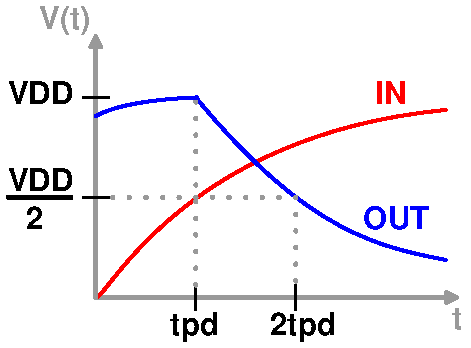
\includegraphics[width=0.8\linewidth]{figs/inv_waves2.pdf}
	            \caption{Inverter waveforms in ring oscillator.}
	            \label{fig:rosc_3stg_wave}
	        \end{subfigure}
	        \caption{Approximate model for ring oscillator inverter delay cell.}
	        \label{fig:rosc_3stg}
	    \end{figure}

		To calculate oscillation frequency ring oscillator from the RC model, several inferences are made:
		\begin{itemize}
			\item The switching point $V_M$ of the inverters is $V_{DD}/2$, based on the assumption that the NMOS and PMOS are of equal strength.
			\item The output of an inverter will have a decaying exponential which starts coincident with the passing of $V_M$ at the input.
			\item The propagation delay $t_{pd}$ for an inverter will be the time differential between the $V_M$ crossing points on the input and output.
			\item The oscillator frequency will be $f_{osc}$ = $1/2Nt_{pd}$, where N is the number of stages (i.e. defined by 2N propagation delays).
		\end{itemize}
			Following the definition of $V_M$, it is trivial to find that $t_{pd}$ = $\tau\ln2$. It is therefore known that:
		\begin{equation}
			f_{osc}^{-1} = 2Nt_{pd} = \frac{2\ln(2)NC}{\langle g_{ch}\rangle}
		\end{equation}

		\subsubsection{Finding $\langle g_{ch}\rangle$ and C}
			The node capacitance C is trivial to find based on the inverter gate capacitance and a lumped load capacitance term $C_L$:
			\begin{equation}
				C = C_{ox}\left ( W_N L_N + W_P L_N \right) + C_L
			\end{equation}
			The average channel conductance $\langle g_{ch} \rangle$ is more involved to find. To do so, several assumptions are made:
			\begin{itemize}
				\item L $>>$ L$_{min}$, so no velocity saturation, and therefore square law is applicable.
				\item NMOS and PMOS have equal $V_t$ and transconducance.
				\item Output transition occur with the active FET in saturation during $t_{pd}$. This requires:
				\begin{itemize}
					\item $V_{DD}/4 < V_{t} < V_{DD}/2$
				\end{itemize}
			\end{itemize}
			Following those assumptions, $\langle g_{ch} \rangle$ can be computed via integral within the period $t_{pd}$:
			\begin{equation}
				\langle g_{ch} \rangle = \frac{1}{t_{pd}} \int_0^{t_{pd}}\frac{I_{out}(t)}{V_{out}(t)}dt
			\end{equation}
			$I_{out}$ is computed using the saturated MOSFET square law model an exponential waveforms assumptions. An $I_{short}$ term is included to account for output current reduction from short-circuit conduction.
			\begin{equation}
				I_{out}(t) = \frac{k_n}{2}\left(\frac{W}{L}\right)_n\left[\left(V_{in}(t) - V_t\right)^2 \right]  - I_{short} = \frac{k_n}{2}\left(\frac{W}{L}\right)_n\left[\left(V_{DD}\left(1-e^{-t/\tau}\right) - V_t\right)^2 - \left(\frac{V_{DD}}{2} -V_t\right)^2\right]
			\end{equation}
			$k_n = \mu_nC_{ox}$, with the equal PMOS/NMOS assumption, $k_n\left(\frac{W}{L}\right)_n=k_p\left(\frac{W}{L}\right)_p$. $V_{out}$ is simply a decaying exponential with a delay $t_pd$ versus the input:
			\begin{equation}
				V_{out} = V_{DD}e^{-(t-t_{pd})/\tau}
			\end{equation}
			Now, computing the integral for $\langle g_{ch} \rangle$ yields:
			\begin{equation}
				\langle g_{ch} \rangle = \frac{1}{2}\mu_nC_{ox}\left(\frac{W}{L}\right)_n\left[V_{DD}\left(\frac{7}{8\ln2}-1\right)-V_t\left(\frac{1}{\ln2}-1\right) \right]
			\end{equation}
			As a simplification, $\alpha$ is defined as:
			\begin{equation}
				\alpha = \left[V_{DD}\left(\frac{7}{8\ln2}-1\right)-V_t\left(\frac{1}{\ln2}-1\right) \right]
			\end{equation}	
		
		\subsubsection{Handling unequal NMOS/PMOS}
			In the case of different threshold voltages for NMOS and PMOS:
			\begin{equation}
				f_{osc}^{-1} = N(t_{pdn} + t_{pdp}) = \ln(2)NC\left(\frac{1}{\langle g_{ch}\rangle_n} + \frac{1}{\langle g_{ch}\rangle_p}\right) = \frac{2\ln(2)NC}{\langle g_{ch}\rangle'}
			\end{equation}	
			A modified $\langle g_{ch}\rangle'$ is defined:
			\begin{align}
				\langle g_{ch}\rangle' = 2\left(\frac{1}{\langle g_{ch}\rangle_n} + \frac{1}{\langle g_{ch}\rangle_p}\right)^{-1} = 2\frac{\langle g_{ch}\rangle_n \langle g_{ch}\rangle_p}{\langle g_{ch}\rangle_n + \langle g_{ch}\rangle_p}
				= 2\frac{\frac{1}{2}\mu_nC_{ox}\left(\frac{W}{L}\right)_n \alpha_n\frac{1}{2}\mu_pC_{ox}\left(\frac{W}{L}\right)_p \alpha_p}{\frac{1}{2}\mu_nC_{ox}\left(\frac{W}{L}\right)_n\alpha_n + \frac{1}{2}\mu_pC_{ox}\left(\frac{W}{L}\right)_p\alpha_p}
			\end{align}	
			This is somewhat unmanagable, hovever enforcing $\mu_nC_{ox}\left(\frac{W}{L}\right)_n = \mu_pC_{ox}\left(\frac{W}{L}\right)_p$ for $V_M$ to equal $V_{DD}/2$ gives:
			\begin{align}
				\langle g_{ch}\rangle' = \frac{1}{2}\mu_nC_{ox}\left(\frac{W}{L}\right)_n\frac{2 \alpha_n\alpha_p}{\alpha_n + \alpha_p} = \frac{1}{2}\mu_nC_{ox}\left(\frac{W}{L}\right)_n \alpha'
			\end{align}	
			Thus $\alpha_n$ and $\alpha_p$ are found for the according threshold voltages and then $\langle g_{ch}\rangle$ can be found.
			\begin{equation}
				\alpha' =  \frac{2 \alpha_n\alpha_p}{\alpha_n + \alpha_p}
			\end{equation}

		\subsubsection{Solving for oscillator frequency and power}
			Solving for oscillator frequency:
			\begin{equation}
				f_{osc} = \frac{\mu_nC_{ox}}{4\ln2NC}\left(\frac{W}{L}\right)_n\left[V_{DD}\left(\frac{7}{8\ln2}-1\right)-V_t\left(\frac{1}{\ln2}-1\right) \right]
			\end{equation}
			If gate capacitance is the dominant load component, and PMOS/NMOS are equal sized such that $C=2WLC_{ox}$:
			\begin{equation}
				f_{osc} = \frac{\mu_n}{8\ln2N}\cdot\frac{1}{L^2}\left[V_{DD}\left(\frac{7}{8\ln2}-1\right)-V_t\left(\frac{1}{\ln2}-1\right) \right]
			\end{equation}
			Power can also be calculated, knowing in digital circuits $P = fC_{\Sigma}V_{DD}^2$, where $C_{\Sigma}$ is the total active capacitance. Thus:
			\begin{equation}
				P_{osc} = Nf_{osc}CV_{DD}^2 = \frac{\mu_nC_{ox}}{4\ln2}\left(\frac{W}{L}\right)_n\left[V_{DD}\left(\frac{7}{8\ln2}-1\right)-V_t\left(\frac{1}{\ln2}-1\right) \right]
			\end{equation}
			It should be noted that the power consumption is proportional to FET aspect ratio (W/L).

	\subsection{Ring oscillator backgate tuning derivation}
		Using the basic expressions for ring oscillator frequency, the operature under backgate biasing can be found. In UTBB-FDSOI processes, the threshold voltage of a FET varies with linear dependence on the applied back gate bias $V_{BG}$ (relative to source). Given the body effect coefficient of a process, $\gamma$, $V_t$ is:
		\begin{equation}
			V_t = V_{t0} - \gamma V_{BG}
		\end{equation}
		Using this in the ring oscillator frequency equation:
		\begin{equation}
			f_{osc} = \frac{\mu_nC_{ox}}{4\ln2NC}\left(\frac{W}{L}\right)_n\left[V_{DD}\left(\frac{7}{8\ln2}-1\right)-V_{t0}\left(\frac{1}{\ln2}-1\right) + \gamma V_{BG}\left(\frac{1}{\ln2}-1\right) \right]
		\end{equation}
		Equivalently, $f_{osc} = f_{0,osc} + \Delta f_{osc}(V_{BG})$, where:
		\begin{equation}
			\Delta f_{osc}(V_{BG}) = \gamma V_{BG}\frac{\mu_nC_{ox}}{4\ln2NC}\left(\frac{W}{L}\right)_n\left[\frac{1}{\ln2}-1\right]
		\end{equation}	
		And $f_{0,osc}$ is the frequency with no backgate bias. If the backgate is swept from 0 to $V_{DD}$, and the node capacitance is increasingly varied (C0 to C3), Figure \ref{fig:rosc_tuning} is observed. Note that the change in frequency is linear with to backgate bias.
		\FloatBarrier
		\begin{figure}[htb!]
			\center\includegraphics[width=0.3\linewidth, angle=0]{figs/backgate_rosc_tuning2.pdf}
			\caption{Backgate-tuned ring oscillator with coarse tuning capacitor bank.}
			\label{fig:rosc_tuning}
		\end{figure}
		If the backgate voltage is constrained in the range [0, $V_{DD}$], the center frequency $f_c$ in the tuning range of the oscillator is then:
		\begin{equation}
			f_{c} = \frac{\mu_nC_{ox}}{4\ln2NC}\left(\frac{W}{L}\right)_n\left[V_{DD}\left(\frac{7}{8\ln2}-1+\frac{\gamma}{2\ln2}-\frac{\gamma}{2}\right)-V_{t0}\left(\frac{1}{\ln2}-1\right)\right]
		\end{equation}
		The tuning range is also therefore:
		\begin{equation}
			\Delta f = \frac{\gamma V_{DD}}{2}\frac{\mu_nC_{ox}}{4\ln2NC}\left(\frac{W}{L}\right)_n\left[\frac{1}{\ln2}-1\right]
		\end{equation}
		The fractional tuning range of the oscillator is:
		\begin{equation}
			\frac{\Delta f}{f_c} = \frac{1}{2}\cdot\frac{\gamma V_{DD}\left( 1-\ln2 \right)}{V_{DD}\left(\frac{7}{8}-\ln2+\frac{\gamma}{2}-\frac{\gamma}{2}\ln2\right)-V_{t0}\left(1-\ln2\right)}
		\end{equation}	
		If a N-bit DAC is used to control the oscillator, the resulting DCO gain is therefore:
		\begin{equation}
			K_{DCO} = \frac{\Delta f}{2^{N_{DAC}}} = \frac{f_c}{2^{N_{DAC}+1}}\cdot\frac{\gamma V_{DD}\left( 1-\ln2 \right)}{V_{DD}\left(\frac{7}{8}-\ln2+\frac{\gamma}{2}-\frac{\gamma}{2}\ln2\right)-V_{t0}\left(1-\ln2\right)}
		\end{equation}	
	\subsection{DCO Gain Uncertainty}
		The DCO gain $K_{DCO}$ is used in setting the loop filter coefficients, so the uncertainty of the DCO gain is of interest to allow for statistical analysis of the PLL across process variation. The uncertainty of $K_{DCO}$ (normalized with nominal $K_{DCO}$ value) as a function of $V_{DD}$, $V_{t0}$ and $\gamma$ is:
		\begin{equation}
			\sigma_{KDCO} = \sqrt{\left(\frac{\partial K_{DCO}}{\partial V_{DD}}\cdot\frac{\sigma_{VDD}}{K_{DCO}} \right)^2 + \left(\frac{\partial K_{DCO}}{\partial V_{t0}}\cdot\frac{\sigma_{Vt0}}{K_{DCO}} \right)^2 + \left(\frac{\partial K_{DCO}}{\partial \gamma}\cdot\frac{\sigma_\gamma}{K_{DCO}} \right)^2}
		\end{equation}

		\begin{align}
			\frac{\partial K_{DCO}}{\partial V_{DD}} &= \frac{f_c}{2^{N_{DAC}+1}}\cdot\frac{-\gamma V_{t0}(1-\ln2)^2}{\left[ V_{DD}\left(\frac{7}{8}-\ln2+\frac{\gamma}{2}-\frac{\gamma}{2}\ln2\right)-V_{t0}\left(1-\ln2\right) \right]^2}\\
			\frac{\partial K_{DCO}}{\partial V_{t0}} &= \frac{f_c}{2^{N_{DAC}+1}}\cdot\frac{\gamma V_{DD}(1-\ln2)^2}{\left[ V_{DD}\left(\frac{7}{8}-\ln2+\frac{\gamma}{2}-\frac{\gamma}{2}\ln2\right)-V_{t0}\left(1-\ln2\right) \right]^2}\\
			\frac{\partial K_{DCO}}{\partial \gamma} &= \frac{f_c}{2^{N_{DAC}+1}}\cdot\frac{V_{DD}\cdot(1-\ln2) \left[ V_{DD}\left(\frac{7}{8}-\ln2\right)-V_{t0}\left(1-\ln2\right) \right]}{\left[ V_{DD}\left(\frac{7}{8}-\ln2+\frac{\gamma}{2}-\frac{\gamma}{2}\ln2\right)-V_{t0}\left(1-\ln2\right) \right]^2}
		\end{align}
		Simplified:
		\begin{multline}
			\sigma_{KDCO} = \frac{1}{\gamma V_{DD} \left[ V_{DD}\left(\frac{7}{8}-\ln2+\frac{\gamma}{2}-\frac{\gamma}{2}\ln2\right)-V_{t0}\left(1-\ln2\right) \right]}\cdot\\ \sqrt{\left(\gamma V_{t0} (1-\ln2)\sigma_{VDD} \right)^2 + \left(\gamma V_{DD} (1-\ln2)\sigma_{Vt0} \right)^2 + \left( V_{DD}\left[ V_{DD}\left(\frac{7}{8}-\ln2\right)-V_{t0}\left(1-\ln2\right) \right]\sigma_{\gamma} \right)^2 }
		\end{multline}		
		\textbf{TODO} - extract $\gamma$, $V_{t0}$ variance for FETs in process kit.



\end{document}